\documentclass[preprint,nocopyrightspace]{sigplanconf}

%\usepackage[T1]{fontenc}
\usepackage{bcprules}
\usepackage{latexsym}
\usepackage{amssymb}
\usepackage{amsmath}
\usepackage{amsthm}
\usepackage{url}
\usepackage{alltt}
\usepackage{graphicx}
\usepackage[dvips]{color}
\usepackage{proof}



\newcommand\TODO[1]{\textcolor{red}{[TODO: {#1}]}}
\newcommand\cc[1]{\textcolor{red}{{#1}}}
\newcommand\memo[1]{\textcolor{red}{[{#1}]}}

\newcommand\widthcoefh{0.23}
\newcommand\widthcoef{0.46}
\newcommand\widthcoefw{0.96}

\chardef\us=`\_

\newcommand\LINT{\mathcal{L}_{int}}
\newcommand\LLIST{\mathcal{L}_{list}}
\newcommand\LREC{\mathcal{L}_{rec}}

\newcommand\ra{\Rightarrow}
\newcommand\red{\longrightarrow}
\newcommand\reds{\red^*}
\newcommand\Red[1]{\longrightarrow_{#1}}
\newcommand\Reds[1]{\Red{#1}^*}

\newcommand\set[1]{\{{#1}\}}
\newcommand\seq[1]{\widetilde{#1}}
\newcommand\CONSTR{C}
\newcommand\Constr[2]{\CONSTR_{#1}({#2})}
\newcommand\WILD{\_\!\_}
\newcommand\OP{\mathrm{op}}
\newcommand\Op[1]{\OP({#1})}
\newcommand\TRUE{\mathit{true}}
\newcommand\FIX{\mathbf{fix}}
\newcommand\Fix[3]{\FIX({#1},{#2},{#3})}
\newcommand\FAIL{\mathbf{fail}}
\newcommand\ASSERT{\mathbf{assert}}
\newcommand\Assert[1]{\ASSERT({#1})}
\newcommand\LIST{\mathbf{list}}
\newcommand\List[1]{{#1}\ \LIST}
\newcommand\NIL{\mathbf{nil}}
\newcommand\CONS{\mathbf{cons}}
\newcommand\Cons[2]{\CONS({#1},{#2})}
\newcommand\LEAF{\mathbf{leaf}}
\newcommand\TREE{\mathbf{tree}}
\newcommand\NODE{\mathbf{node}}
\newcommand\Node[2]{\NODE({#1},{#2})}
\newcommand\RTREE{\mathtt{rtree}}
\newcommand\RTLIST{\mathtt{rtreelist}}
\newcommand\RTNODE{\mathtt{RTNode}}
\newcommand\RTNIL{\mathtt{RTNil}}
\newcommand\RTCONS{\mathtt{RTCons}}
\newcommand\App[2]{{#1}\,{#2}}
\newcommand\IF{\mathbf{if0}}
\newcommand\THEN{\mathbf{then}}
\newcommand\ELSE{\mathbf{else}}
\newcommand\If[3]{\IF~{#1}~\THEN~{#2}~\ELSE~{#3}}
\newcommand\Pair[2]{({#1},{#2})}
\newcommand\FST{\mathbf{fst}}
\newcommand\SND{\mathbf{snd}}
\newcommand\Fst[1]{\App{\FST}{#1}}
\newcommand\Snd[1]{\App{\SND}{#1}}
\newcommand\MATCH{\mathbf{match}}
\newcommand\WITH{\mathbf{with}}
\newcommand\Match[3]{\MATCH\ {#1}\ \WITH\ \NIL \ra {#2} \mid \Cons{x_1}{x_2} \ra {#3}}
\newcommand\MatchRec[3]{\MATCH\ {#1}\ \WITH\ \Constr{1}{\widetilde{x_1}} \ra {#2} \mid \dots \mid \Constr{k}{\widetilde{x_k}} \ra {#3}}
\newcommand\Abs[2]{\lambda{#1}.\,{#2}}
\newcommand\AbsC[2]{\lambda^{C}{#1}.\,{#2}}
\newcommand\AbsN[2]{\lambda^{N}{#1}.\,{#2}}
\newcommand\AbsT[3]{\lambda{#1}\COL{#2}.\,{#3}}
\newcommand\AbsL[4]{\lambda^{#1}{#2}\COL{#3}.\,{#4}}
\newcommand\AbsTC[3]{\AbsL{C}{#1}{#2}{#3}}
\newcommand\AbsTN[3]{\AbsL{N}{#1}{#2}{#3}}
\newcommand\LET{\mathbf{let}}
\newcommand\IN{\mathbf{in}}
\newcommand\Let[3]{\LET\ {#1} = {#2}\ \IN\ {#3}}
\newcommand\UNIT{\mathbf{unit}}
\newcommand\INT{\mathbf{int}}
\newcommand\TFun[2]{{#1}\mathbin{\rightarrow}{#2}}
\newcommand\TPair[2]{{#1}\mathbin{\times}{#2}}

\newcommand\subst[2]{{#1}/{#2}}

\newcommand\FV[1]{\mathit{FV}({#1})}

\newcommand\Trans[1]{[\![{#1}]\!]}
\newcommand\TransRec[2]{[\![{#2}]\!]_{#1}}
\newcommand\Denote[1]{[\![{#1}]\!]}
\newcommand\RecConstr[5]{\mathit{Constr}({#1},{#2},{#3},{#4},{#5})}
\newcommand\RecDestr[4]{\mathit{Destr}({#1},{#2},{#3},{#4})}
\newcommand\RecDestrBase[4]{\mathit{Destr'}({#1},{#2},{#3},{#4})}

\newcommand\ExpNRec[2]{[\![{#2}]\!]_{#1}}
\newcommand\COL{\mathbin{:}}
\newcommand\p\vdash
\newcommand\Exp[3]{{#1} \p {#2} \Rightarrow {#3}}
\newcommand\CPSty[1]{[\![{#1}]\!]}
\newcommand\CPS[5]{{#1} \p {#2} \COL {#3}, {#4} \leadsto {#5}}
\newcommand\CPSprog[3]{{#1} \p {#2} \leadsto {#3}}

\newcommand\TFunL[3]{{#2}\mathbin{\rightarrow^{#1}}{#3}}
\newcommand\TFunN[2]{\TFunL{N}{#1}{#2}}
\newcommand\TFunC[2]{\TFunL{C}{#1}{#2}}
\newcommand\MApp[2]{\,{#1}\mathbin{\overline@}{#2}}
\newcommand\MAbs[2]{\overline\lambda{#1}.\,{#2}}

\newcommand\IC{C}
\newcommand\NC{N}
\newcommand\AT{\mathit{X}}

\newcommand\Abst[5]{{#1} \mid {#2} \vdash {#3} : {#4} \leadsto {#5}}
\newcommand\AbstPLDI[4]{{#1} \vdash_{\texttt{NS}} {#2} : {#3} \leadsto {#4}}
\newcommand\AbstProg[4]{{#1} \mid {#2} \vdash {#3} \leadsto {#4}}
\newcommand\Affine[2]{\mathit{Affine}{({#1}, {#2})}}
\newcommand\AffineT[3]{\mathit{Affine}{({#1}, {#2}, {#3})}}

\newcommand\Br[2]{{#1}\mathbin{\blacksquare}{#2}}

\newcommand\AbstLoc[2]{\langle{#1}\rangle_{#2}}
\newcommand\Dom[1]{\mathit{dom}(#1)}
\newcommand\call{\prec}
\newcommand\main{\mathit{main}}
\newcommand\SApp[3]{\mathit{App}^{#1}({#2},{#3})}
\newcommand\NCAdd[2]{{#1}\mathbin{\oplus}{#2}}


\begin{document}

\conferenceinfo{PEPM '13}{January, Roma.}
\copyrightyear{2013}
\copyrightdata{[to be supplied]}

\title{Towards a Scalable Software Model Checker for Higher-Order Programs}

\authorinfo{Ryosuke Sato}
           {Tohoku University}
           {ryosuke@kb.ecei.tohoku.ac.jp}
\authorinfo{Hiroshi Unno}
           {University of Tsukuba}
           {uhiro@cs.tsukuba.ac.jp}
\authorinfo{Naoki Kobayashi}
           {University of Tokyo}
           {koba@is.s.u-tokyo.ac.jp}

\maketitle

\begin{abstract}
In our recent paper, we have shown how to construct a fully-automated
program verification tool (so called a ``software model checker'') for a
tiny subset of functional language ML, by combining higher-order model
checking, predicate abstraction, and CEGAR.  This can be viewed as a
higher-order counterpart of previous software model checkers for
imperative languages like BLAST and SLAM.  The na\"{\i}ve application of
the proposed approach, however, suffered from scalability problems, both
in terms of efficiency and supported language features.  To obtain more
scalable software model checkers for full-scale functional languages, we
propose a series of optimizations and extensions of the previous
approach. Among others, we introduce (i) selective CPS transformation,
(ii) selective predicate abstraction, and (iii) refined predicate
discovery as optimization techniques; and prpose (iv) functional encoding of
recursive data structures and control operations to support a larger
subset of ML.  We have implemented the proposed methods, and obtained
promising results.
%%%Higher-order model checking has been studied recently, and applied to
%%%verification of higher-order functional programs.  In previous work, we
%%%have developed an automated verifier for functional programs. The
%%%verification framework, however, have the following problems: (i) it is
%%%not scalable in a na\"{\i}ve way, and (ii) it cannot directly deal with
%%%recursive data types (e.g., lists and trees) and control operators
%%%(e.g., exceptions and call/ccs), which are necessary to practical
%%%functional languages.
%%%
%%%In this paper, to overcome these problems, we extend and refine the
%%%verification framework in the following way. First, we formalize
%%%functional encoding of recursive data types and control operators.
%%%Second, we define techniques of selective CPS transformation and reduced
%%%abstraction.  We have implemented a prototype verifier for functional
%%%programs based on the framework and tested for several programs.
\end{abstract}



%\section{Introduction}
%[background]
%
%[Show running example of verifying a program with lists]
%
%[discovering general predicates]
%
%[Show running example of expanding non-recursive functions]
%
%[the overview of this framework]
%
%\section{Language}
% [Introduction of the target language (= list constructor/destructor + language of PLDI2011 + pairs.)]
%
%\section{Model Checking for Higher-order Programs with Integers}
% [Introduction of language (of PLDI2011 + pairs.)]
%
% [Description of the framework of PLDI2011.]
%
%\section{Optimization}
%\subsection{Inlining Non-recursive Function}
% [Show an example of the verification with inlining]
%
%\subsection{Selective CPS Transformation}
% [Show an example of the selective CPS transformation]
%
%\section{Functional Encoding of Lists}
% [Show how to encode lists, and how to translate the program with lists]
%\subsection{Extensions for Recursive Data Structures}
% [Show how to encode other data structures]
%
%\section{Extension for Control Operators}
% [Introduce language with control operators (exceptions, call/cc, etc.), and just to say ``Just to do CPS transformation'']
%
%\section{Implementation and Preliminary Experiments}
%
%\section{Related work}
% [Comparison with container abstraction (Dillig et al. POPL11, etc.)]
%
% [Comparison with verification of functional programs with data structures (liquid types, sized types, HMTT, PMRS, etc.)]
%
% [Comparison with others (Soonho Kong et al. APLAS10, etc.)]
%
%\section{Conclusion}
%
%


%\category{D.2.4}{Software Engineering}{Software/Program Verification}
%\category{F.3.1}{Logics and Meanings of Programs}{Specifying and Verifying and Reasoning about Programs}
%
%\terms
%Verification, Algorithm, Language
%
%\keywords
%Higher-Order Model Checking,
%Predicate Abstraction, Abstraction Refinement,
%Dependent Types, CPS Transformation

\section{Introduction}
\label{sec:intro}

In our recent paper~\cite{KobayashiPLDI2011}, we have shown how to
construct a fully-automated program verification tool (so called a
``software model checker'') for a tiny subset of functional language ML, a
simply-typed lambda calculus with recursion and integers.
The framework is an extension of higher-order model checker
(more precisely, the model checker for higher-order recursion scheme)
for infinite data domains such as integers by the techniques of
predicate abstraction and CEGAR.  This can be viewed as a higher-order
counterpart of previous software model checkers for imperative languages
like BLAST~\cite{Henzinger2002} and SLAM~\cite{Ball2002}.
We have implemented a verification tool, MoCHi, based on the framework.

The na\"{\i}ve application of the proposed approach, however, suffered
from scalability problems, both in terms of efficiency and supported
language features. For example, the previous framework does not support
recursive data structures and our implementation based on the framework
does not support control operations.  To explain the problem of the
previous framework/implementation, let us first review our previous
framework.

Our previous verification framework~\cite{KobayashiPLDI2011} is based on
predicate abstraction and CEGAR for a higher-order model checker.
Figure~\ref{fig:cegar} shows the overall structure of our previous
method.  First, an input program, written in a simply typed call-by-value
lambda calculus with recursion and integers, is abstracted to a
higher-order boolean program by predicate abstraction in Step 1.  The
abstracted program is verified by a higher-order model checker, where
models are described by higher-order recursion schemes, in Step 3.
Higher-order recursion schemes can be viewed as a simply typed
call-by-name lambda calculus with finite data domains and recursion.  To
resolve the gap between the evaluation strategies of higher-order
recursion schemes and higher-order boolean programs, we translate
the call-by-value program into a call-by-name program in Step 2. If the
abstracted program is safe, the original functional program is also safe.  If not, we
check whether the original program is in fact unsafe or the abstraction is too coarse
in Step 4. If the latter, we discover new predicates in Step 5.  We
repeat these steps until we find whether the program is safe or not.
%Our previous verification framework is a CEGAR-based one on higher-order
%model checker.  The verification proceeds as follows.  First, an input
%program, written in simply typed call-by-value lambda calculus with
%integers, is abstracted to a higher-order boolean program by predicate
%abstraction.  The abstracted program is verified by higher-order model
%checker. Higher-order model checker is the model checker for
%higher-order recursion schemes, it can be viewed as a simply typed
%call-by-name lambda calculus.  Here, to resolve the gap between
%semantics of higher-order recursion schemes and higher-order boolean
%programs, we need to translate call-by-value programs into call-by-name
%programs.  The abstracted program translated by CPS transformation is
%checked by the model checker. If the abstracted program is safe, the
%source program is also safe.  Otherwise, the model checker generates a
%counterexample for the abstracted program.  We can find a corresponding
%concrete error trace from the counterexample, and we can check whether
%the error path is feasible or not in the source program by symbolic
%execution.  If the error trace is feasible, the source program is
%unsafe.  Otherwise, the abstraction is too coarce to verify the source
%program.  We next discover new predicates to refute the
%counterexample, and repeat the above processes until we find out whether
%the program is safe or not.

\begin{figure}[tp]
 \begin{center}
  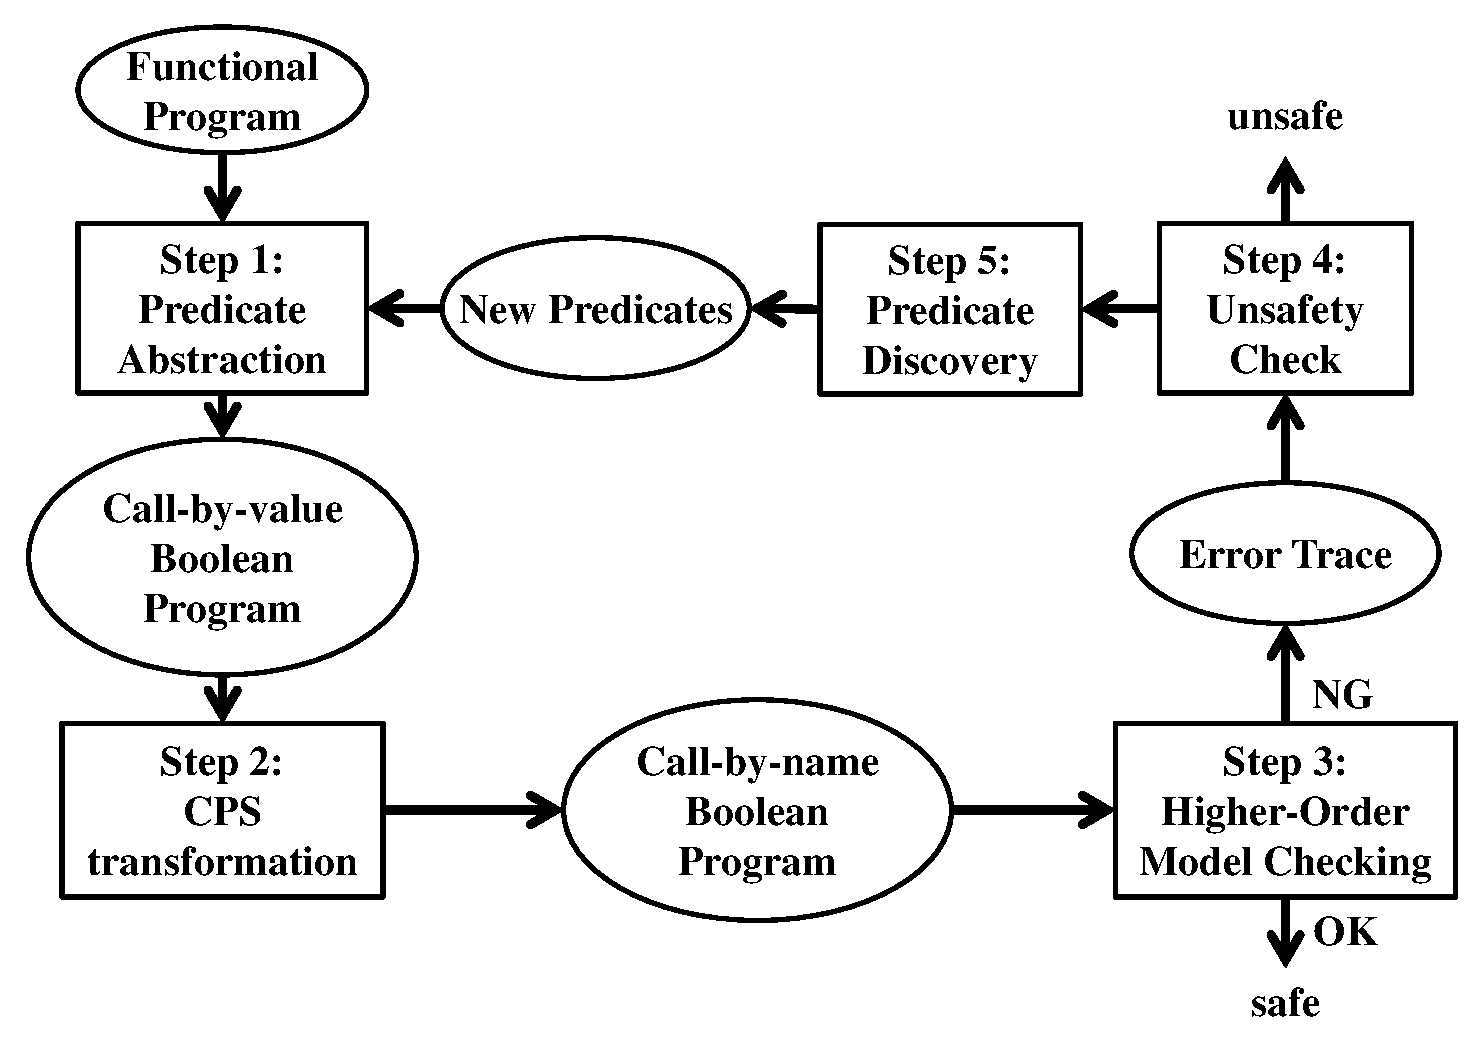
\includegraphics[scale=0.4]{overall.eps}
 \end{center}
\caption{Higher-Order Model Checking with Predicate Abstraction and CEGAR}
\label{fig:cegar}
\end{figure}

%The na\"{\i}ve application of the proposed approach, however, suffered
%from scalability problems, both in terms of efficiency and supported
%language features.  The verification framework supports infinite data
%domains other than integers.  However, we need interpolant theorem
%provers that can deal with the each infinite data domains (e.g., lists
%and trees).  Moreover, the verification framework does not support
%control operations (e.g., exceptions and call/cc).

%The na\"{\i}ve application of the proposed approach, however, suffered
%from scalability problems, both in terms of efficiency and supported
%language features.
%In this paper, we address the following
%problems of our previous work.
%\begin{enumerate}
% \item The previous framework requires an appropriate set of predicates for all
%       functions in the source program of predicate abstraction.
% \item Na\"{\i}ve CPS transformation extremely increases the computational cost
%       of model checking of higher-order boolean program because of the
%       increase of the order of the program.
% \item The previous framework does not support recursive data
%       structures like lists and trees.  Moreover, the previous
%       implementation does not support control operations like
%       exceptions and call/cc.
%\end{enumerate}
%
%We discuss each problem in more detail and explain our approach below.

In this paper, we address three problems of our previous work.
We discuss each problem and explain our approach below.

\begin{enumerate}
\item The main bottleneck of the previous version of MoCHi was the
      predicate abstraction and discovery (Steps 1 and 5), rather than
      higher-order model checking. Our previous method for predicate
      abstraction tried to abstract every integer argument of a function
      to a tuple of booleans.  As a result, verification of a program did
      not succeed until an appropriate set of predicates is found for
      \emph{every} function in the program.  For example, consider the
      program shown in Fig.~\ref{fig:sum}.  The program can be successfully
      verified if we abstract the program by using predicates
      $\Abs{y}{y \geq 0}$ for the second argument of \texttt{add} and
      $\Abs{r}{r \geq x}$ for the return value of \texttt{add} and
      \texttt{sum}.  The following is the
      abstracted program using the above predicates.

\begin{figure}[t]
\begin{alltt}
let add x y = x + y
let rec sum x = if x <= 0 then 0 else add x (sum (x-1))
let main x = assert (sum x >= x)
\end{alltt}
\caption{Example Program for Selective Predicate Abstraction}
\label{fig:sum}
\end{figure}
\begin{alltt}
let add () b = b
let rec sum () = if * then true
                else add (if sum () then true else *)
let main x = assert (sum ())
\end{alltt}
      Here, ``*'' means a non-deterministic boolean
      value.  The argument \texttt{b} denotes whether $\mathtt{y} \geq 0$ or not.
      Automatically finding all such appropriate predicates is
      difficult.  In the previous paper~\cite{KobayashiPLDI2011}, we
      have adapted CEGAR to find such predicates, but the technique is
      necessarily heuristic, and often fails.  If we abstract the
      program using only the predicate $\Abs{r}{r \geq x}$ for the return
      value of \texttt{sum}, we get the following abstracted program.
\begin{alltt}
let add () () = ()
let rec sum u = if * then true
                else let b = sum () and u = add () () in
                       *
let main x = assert (sum ())
\end{alltt}
      Since the return value of \texttt{add} is non-informative, the
      abstraction is too coarse.

      To reduce the burden to the predicate discovery phase, we introduce
      a refinement of predicate abstraction called \emph{selective
      predicate abstraction}.  As the name suggests, the selective
      predicate abstraction applies predicate abstraction to only a
      certain set of functions, and avoids abstraction of the other
      functions by inlining them.  The selective predicate abstraction
      generates the following safe program by using only the
      predicate $\Abs{r}{r \geq x}$ for the return values of \texttt{sum}
      and inlining \texttt{add}.
\begin{alltt}
let rec sum () = if * then true else if sum () then true else *
let main () = assert (sum ())
\end{alltt}
      In this way the selective predicate abstraction improves the
      precision of abstraction and reduce the cycle of CEGAR.

%%The first problem increases the number of CEGAR-cycle.
%To see the first problem, consider the following program.
%\begin{alltt}
%let add x y = x + y
%let rec sum x = if x < 0 then 0 else add x (sum (x-1))
%let main x = assert (sum x >= 0)
%\end{alltt}
%In our previous framework, we have to give predicate $\Abs{x}{x\geq0}$
%for return values of \texttt{sum}, return values of \texttt{add}, and
%arguments of \texttt{add}.  The following is the abstracted program
%using the predicate.
%\begin{alltt}
%let add bx by = if bx \&\& by then true else rand_bool()
%let rec sum _ = if rand_bool() then true
%                else add true (sum ())
%let main x = assert (sum ())
%\end{alltt}
%Here, \texttt{bx} is true and \texttt{bx} is true denote that
%$\mathtt{x} \geq 0$ and $\mathtt{y} \geq 0$, respectively.
%%If we abstract the program using predicate
%%$\Abs{x}{x\geq0}$ for return values of function \texttt{sum}, we get the
%%following abstracted program.
%%\begin{alltt}
%%let add u1 u2 = ()
%%let rec sum u = if rand_bool() then true
%%                else let b = sum () in
%%                     let u = add () () in
%%                       rand_bool()
%%let main x = assert (sum ())
%%\end{alltt}
%\texttt{rand\us{}bool()} means a non-deterministic boolean value.
%In fact, we can abstract the source program to the following program by
%using the definition of \texttt{add} with predicate $\Abs{x}{x\geq0}$
%only for return values of \texttt{sum}.
%\begin{alltt}
%let rec sum _ = if rand_bool() then true
%                else if sum () then true else rand_bool()
%let main x = assert (sum ())
%\end{alltt}
%In the body of \texttt{sum}, \texttt{add x (sum (x-1))}, i.e. \texttt{x
%+ sum (x-1)}, is abstracted to \texttt{if sum () then true else rand\us{}bool()}
%because $\mathtt{sum ()}$ is true denotes $\mathtt{sum (x-1)} \geq 0$.
%The case of $\mathtt{b}=\mathtt{false}$ is similar.
%We distinguish functions that are abstracted from functions that is not abstracted.
%In the example above, functions \texttt{sum} and \texttt{main} are abstracted, and
%function \texttt{add} is not abstracted.
%We abstract programs, intuitively, with extracting functions which is not abstracted.
%We formalize this abstraction, called selective predicate abstraction.

\item Another efficiency problem is caused by CPS transformation.  As
      stated above, our approach needs CPS transformation to resolve the
      gap between the evaluation strategies of higher-order recursion schemes and
      higher-order boolean programs.  However, CPS transformation increases the
      order\footnote{The order of program $t$ is the maximum order of
      the types of functions in $t$.  The order of type $\tau$ is
      defined by $\mathit{order}(\INT)=0$,
      $\mathit{order}(\TFun{\tau_1}{\tau_2}) =
      \mathit{max}(\mathit{order}(\tau_1)+1, \mathit{order}(\tau_2))$.}
      of programs and the growth of the order is not bounded by a constant.
      Since the complexity of model checking of higher-order recursion
      scheme is $n$-EXPTIME complete for order-$n$ recursion scheme, the
      increase of the order of an input is crucial to the verification
      time.
%
      For example, consider the following program.
\begin{alltt}
let rec check x f = f x; check (x+1) f
let f x = assert (x >= 0)
let main n = check n f
\end{alltt}
%Function \texttt{check} may cause an assertion failure only when two arguments are given.
      The above program is translated into the following program by
      a na\"{\i}ve call-by-value CPS transformation~\cite{Plotkin1975}.
\begin{alltt}
let rec check x k1 = k1 (\(\lambda\)f.\(\lambda\)k2.f x (\(\lambda\)_.check (x+1) (\(\lambda\)g.g f k2)))
let f x k = assert (x >= 0); k ()
let main n k = check n (\(\lambda\)g. g f k)
\end{alltt}
      To preserve the evaluation order of an original call-by-value program,
      each function of the translated call-by-name program takes
      a continuation and passes its return value to the continuation.  Note here that the
      order of the translated program is increased to 5.
%\begin{alltt}
%let check x k1 = k1 (\(\lambda\)y.\(\lambda\)k2. assert (x = y); k2 ())
%let main k = check (\(\lambda\)f. f n k)
%\end{alltt}
%let apply x k1 = k1 (\(\lambda\)f.\(\lambda\)k2. f x k2)
%let check x k1 = k1 (\(\lambda\)y.\(\lambda\)k2. assert (x = y); k2 ())
%let main n k = check n (\(\lambda\)f1. apply n (\(\lambda\)f2. f2 f1 k))
      We can, however, obtain the following order-3 program instead by omitting the continuation \texttt{k1} of \texttt{check},
      which is actually unnecessary since a partial application of \texttt{check} in the original program never causes side effects including an assertion failure.
\begin{alltt}
let rec check x f k = f x (\(\lambda\)_.check (x+1) f k)
let f x k = assert (x >= 0); k ()
let main n k = check n f k
\end{alltt}
%This transformation uses the fact that the application to the first
%argument does not cause an assertion failure and the context of
%\texttt{call n} is not required to have a continuation.
      Our CPS transformation avoids such unnecessary insertions of
      continuations.  We formalize this transformation, called
      \emph{selective CPS transformation}.

%Higher-order model checking (more precisely, the model
%checking of higher-order recursion schemes) has been studied
%recently~\cite{Ong2006}, and applied to verification of higher-order
%functional programs~\cite{KobayashiPOPL2009,KobayashiPLDI2011}.  Our
%previous framework~\cite{KobayashiPLDI2011} can verify higher-order
%programs.  The framework, however, cannot deal with recursive data
%structures, which are necessary for practical functional languages.
%Moreover, the na\"{\i}ve implementation based on the framework cannot
%verify large programs.
%
%In this paper, we introduce extensions and optimizations of the
%verification framework.  The extensions are language extensions to deal
%with recursive data structures (e.g., lists and trees) and control
%operators (e.g., exceptions and call/cc).  Our approach is to translate
%a source program written in the extended language to a program written
%in the previous language. This translation is sound and complete.

%The goal of the verification is to check
%that all assertions in a program never fail and pattern matching
%failures do not occur.

%\memo{The problem of the previous predicate abstraction}
%we introduce selective predicate abstraction as an optimization technique
%
%\memo{The problem of the previous model checking}
%we introduce selective CPS transformation as an optimization technique
%
%\memo{for language extension}
%(iii) functional encoding of recursive data structures and control operations to support a larger subset of ML.

\item The third problem is the insufficiency of supported language
      features.  Our previous framework requires an
      automated interpolating theorem prover for predicate abstraction and
      discovery, but practical provers are not available for recursive data
      structures like lists and trees. Thus, the implementation dealt with
      only integers as infinite data domains.
      
      To support recursive data structures without relying on interpolating
      theorem provers for them, we extend our verification framework as follows.
      As a preprocessing of our CEGAR-based model checking,
      we translate programs that manipulate recursive data structures into ones that manipulate only integers.
      The transformation is carried out by encoding recursive data structures using higher-order functions.  For example, a list is
      encoded to a function that maps an index $i$ to the $i$-th element.
      In a similar way, we support control operations (e.g., exceptions and call/cc) by using higher-order functions.
\end{enumerate}

%Our contributions are (i) the formalization of selective predicate
%abstraction using a simple but effective way to overcome the first
%efficiency problem, (ii) the formalization of selective CPS
%transformation to overcome the efficiency second problem, (iii) the
%formalization for language extension for recursive data structures
%(e.g., lists and trees) and control operations (e.g., exceptions and
%call/cc) that is sound, complete, and general for verification
%frameworks for higher-order language, and (iv) the implementation and
%experiments.

The rest of this paper is organized as follows. 
%In Sect.~\ref{sec:model-check}, we introduce our previous framework for
%higher-order programs with integers, which is the base of our framework
%described in this paper.
We first formalize the source language of verification in
Sect.~\ref{sec:language}.  Section~\ref{sec:opt} formalizes the
selective predicate abstraction and the selective CPS transformation.
Section~\ref{sec:extension} shows the language extensions for recursive
data structures and control operations.  Section~\ref{sec:experiments}
reports experiments.  Section~\ref{sec:related} discusses related work
and Sect.~\ref{sec:conclusion} concludes the paper.














%\section{Introduction}
%\label{sec:intro}
%[background]
%
%In this paper, we propose the verification method for program with
%recursive data types and control operator.  The goal of the verification
%is to check that a program does not execute the command \texttt{fail}.  We can
%also check that pattern matching failures and uncaught exceptions do not
%occur by a trivial transformation. For example, a program
%\texttt{(match t with ...)} cause a pattern match failure if and only if 
%a program \texttt{(match t with ... | \_ -> fail)} execute \texttt{fail}.
%
%The base of our framework is the verification of higher-order programs with integers.
%
%The idea of this framework is to translate a target program (with
%recursive data structures and exceptions) to a higher-order program with
%integers.  For example, the lists $[2;3;5]$ is encoded to a pair of the length $3$
%and a function $f$ such that $f(1)$, $f(2)$, $f(3)$ returns $2$, $3$,
%$5$, respectively.
%A function which takes lists and/or returns lists is encoded to
%a higher-order function which takes functions and/or returns functions.
%
%[Show running example of verifying a program with lists.]
%
%[discovering general predicates]
%
%[Show running example of discovering general predicates.]
%
%
%[the overview of this framework]
%
%We formalize the verification method for a language with lists.
%The verification for recursive data structures are argue in the Section ...
%
%The rest of this paper is organized as follows. We first formalize the
%target language in Section~\ref{sec:target-language}.  In
%Section~\ref{sec:model-check}, we introduce our previous framework for
%higher-order program with integers, which is the base of our framework
%described in this paper.  Section~\ref{sec:encoding} shows the program
%transformation which generate a program without lists from a program with lists,
%and argue about recursive data structures.
%Section~\ref{sec:control} shows that how to deal with control operators.
%Section~\ref{sec:discover}.
%Section~\ref{sec:experiments} reports preliminary experiments.
%Section~\ref{sec:related} discusses related work and
%Section~\ref{sec:conclusion} concludes the paper.
%

%\section{Background: Predicate Abstraction and CEGAR for Higher-order Model Checking}
\label{sec:model-check}
%\memo{Explanation of previous work}
%\cc{
%A source program is translated into a higher-order program with integers
%by encoding recursive data structures. 
%The language for programs with integers is essentially the same as the source
%language in the previous section, except that it has no list constructors and destructors.
%}
We use our previous verification framework for higher-order
programs with integers~\cite{KobayashiPLDI2011}.  This framework is
based on the higher-order model
checking~\cite{Ong2006,KobayashiPOPL2009}, i.e. model checking of
higher-order recursion schemes, with techniques of predicate abstraction
and counter-example guided abstraction refinement for higher-order
functional programs.

Figure~\ref{fig:cegar} shows the overall structure of our previous
method.  We first translate the source program into boolean program by
predicate abstraction.  Here, predicates are given by the notion of
abstraction types.  Abstraction types are simple types with predicates
that is used as how programs are abstracted to boolean programs.  For
example, abstraction type
$\TFun{x\COL\INT[P_1,\dots,P_n]}{r\COL\INT[Q_1,\dots,Q_m]}$ denotes the
return values are abstracted by predicates $Q_1,\dots,Q_m$ assuming
argument are abstracted by predicates $P_1,\dots, P_n$.  We can verify
the abstracted program by using higher-order model checker.
Higher-order model checker, however, cannot be applied directly to the
abstracted program because of the gap between the semantics of the
abstracted program and recursion scheme that has a call-by-name
semantics.  To resolve the gap, we transform the abstracted program into
a CPS program.  The source program is safe if the abstracted program is
safe.  Otherwise, the model checker generates a counterexample for the
abstracted program.  We can find a corresponding concrete error trace,
and we can check the error path is feasible or not in the source program
by symbolic execution.  The source program is unsafe if the error trace
is feasible.  Otherwise, we can know that the abstraction is too coarse
to verify the source program.  We next refine abstraction types to
refute the counterexample, and continue the CEGAR-loop.

We do not show the details of predicate abstraction and CEGAR for higher-order functional programs here.
See the previous paper~\cite{KobayashiPLDI2011} for the details.


%\section{Model Checking for Higher-order Programs with Integers}
%\label{sec:model-check}
%[Introduction of language (of PLDI2011 + pairs.)]
%
%A source program is translated to a higher-order programs with integers
%by encoding lists as functions. The language of essentially the same as the source
%language in the previous section, except that lists constructor and destructor are not in $\LINT$.
%
%[Description of the framework of PLDI2011.]
%
%We can use the verification framework for higher-order programs with integers [refs].


\section{Source Language}
\label{sec:language}
In this section, we introduce the source language of our verification method.
%We extend the language for recursive data structures later.
%As mentioned in Section~\ref{sec:intro}, 
%We formalize the verification method for a language with lists.
%and argue about recursive data structures later.
%Here, we formalize a language for lists. We extend the language for
%recursive data structures later.

The source language is a simply-typed call-by-value higher-order
functional language with recursion and integers (a la ``PCF'') with the
syntax shown in Fig.~\ref{fig:source-syntax}.
%  A program consists a set of top-level functions.
The meta-variable $\OP$ ranges over the sets of operators over integers.
The expressions are standard except that there is a primitive $\FAIL$
that aborts a program.  We use $\TRUE$ and $\FALSE$ as aliases of $0$
and $1$, and we write $\Assert{t}$ for $\If{t}{0}{\FAIL}$,
$(\Abs{x}{t_1})\ t_2$, and $(v_1\ \OP\ v_2)$ for $\Op{v_1,v_2}$.  We
assume that a program is well-typed in the standard simple type system,
where the set of types is given in Fig.~\ref{fig:source-syntax}, and
every function in a program $D$ has a function type and $D$ contains a
distinguished function symbol $\main \in \set{f_1,\dots,f_n}$ whose type
is $\TFun{\INT}{\INT}$.

\begin{figure}[t]
\begin{minipage}{\widthcoef\textwidth}
\[
\begin{array}{lrl}
D\text{ (programs)} &::=& \{f_1 = v_1, \dots, f_n = v_n\} \\
t\text{ (terms)}
  &::=& n \mid x \mid \Abs{x}{t} \mid t_1\ t_2 \mid \Op{v_1,\dots,v_n} \mid \If{t_1}{t_2}{t_3} \mid \FAIL \\
v\text{ (values)} &::=& n \mid x \mid \Abs{x}{t} \\
\tau\text{ (types)} &::=& \INT \mid \TFun{\tau_1}{\tau_2} \\
\end{array}
\]
\end{minipage}
\caption{The syntax of source language}
\label{fig:source-syntax}
\end{figure}

The goal of our verification is to check whether $\App{\main}{n}
\reds_D \FAIL$ for all integers $n$.

%\begin{figure}[t]
%\begin{minipage}{\widthcoef\textwidth}
%\[
%\begin{array}{lrl}
%D\text{ (programs)} &::=& \{f_1 = v_1, \dots, f_n = v_n\} \\
%t\text{ (terms)}
%  &::=& n \mid x \mid \Abs{x}{t} \mid t_1\ t_2 \mid \Op{v_1,\dots,v_n} \mid \If{t_1}{t_2}{t_3} \\
% &\mid& \FAIL \mid \Pair{v_1}{v_2} \mid \Fst{t} \mid \Snd{t} \mid \NIL \mid \Cons{v_1}{v_2} \\
% &\mid& (\MATCH\ {t_1}\ \WITH\ \NIL \ra {t_2} \mid \Cons{x_1}{x_2} \ra {t_3}) \\
%
%v\text{ (values)}
%  &::=& n \mid \Abs{x}{t} \mid \Pair{v_1}{v_2} \mid \NIL \mid \Cons{v_1}{v_2} \\
%
%E\text{ (eval. ctx.)}
%  &::=& [\,] \mid E\ t \mid \App{\Abs{x}{t}}{E} \mid \If{E}{t_2}{t_3} \mid \Fst{E} \mid \Snd{E} \\
% &\mid& (\Match{E}{t_2}{t_3}) \\
%
%\tau\text{ (types)} &::=& \INT \mid \TFun{\tau_1}{\tau_2} \mid \TPair{\tau_1}{\tau_2} \mid \List{\tau} \\
%\end{array}
%\]
%\end{minipage}
%\caption{The syntax of source language}
%\label{fig:source-syntax}
%\end{figure}


%\begin{figure}[t]
%\begin{minipage}{\textwidth}
%  \infrule[E-Var]{(f,t) \in D}{f \Red{D} t}
%
%\medskip
%
%  \infax[E-App]{\App{(\Abs{x}{M})}{v} \Red{D} [x \mapsto v]t}
%
%\medskip
%
%  \infax[E-Op]{\Op{v_1,\dots,v_n} \Red{D} \Denote{\OP}(v_1,\dots,v_n)}
%
%\medskip
%
%  \infax[E-If-Then]{\If{0}{t_1}{t_2} \Red{D} t_1}
%
%\medskip
%
%  \infrule[E-If-Else]{n \neq 0}{\If{n}{t_1}{t_2} \Red{D} t_2}
%
%\medskip
%
%  \infax[E-Fst]{\Fst{\Pair{v_1}{v_2}} \Red{D} v_1}
%
%\medskip
%
%  \infax[E-Snd]{\Snd{\Pair{v_1}{v_2}} \Red{D} v_2}
%
%\medskip
%
%  \infax[E-Match-Nil]{\Match{\NIL}{t_2}{t_3} \Red{D} t_2}
%
%\medskip
%
%  \infax[E-Match-Cons]{\Match{\Cons{v_1}{v_2}}{t_2}{t_3} \Red{D} t_3[\subst{x_1}{v_1}][\subst{x_2}{v_2}]}
%
%\medskip
%
%  \infrule[E-Context]{t \Red{D} t'}{E[t] \Red{D} E[t']}
%
%\medskip
%
%  \infax[E-Fail]{E[\FAIL] \Red{D} \FAIL}
%\end{minipage}
%\caption{The semantics of source language}
%\label{fig:source-semantics}
%\end{figure}




\subsection{Selective CPS transformation}
\label{sec:CPS}
%\TODO{Add discussion about the increase of the order of programs}

This section formalizes selective CPS transformation for abstracted
programs.  As stated in Sect.~\ref{sec:intro}, the idea of the selective
CPS transformation is to distinguish whether a continuation parameter
should be inserted to each expression or not based on whether it has a
side-effect.  When a function application has no side-effects, we need
not insert a continuation.  Here, $\FAIL$,
non-deterministic branch, and non-termination are considered as
side-effects.
%For example, since an
%application of function $\Abs{x}{\Abs{y}{\Assert{x+y}}}$ to a value has
%no side-effects, it can be transformed to CPS by inserting only one
%continuation like $\Abs{x}{\Abs{y}{\Abs{k}{\App{k}{(x+y)}}}}$ instead of
%$\Abs{x}{\Abs{k}{\App{k}{(\Abs{y}{\Abs{k'}{\App{k'}{(x+y)}}})}}}$.

Note that a similar transformation has been proposed by
Nielsen~\cite{Nielsen2001}.  The transformation does not fit our purpose
to translate call-by-value programs into equivalent call-by-name
programs.  A non-terminating program may be transformed into a
terminating (call-by-name) program by their transformation.
%The reason is that programs obtained by their transformation do not
%yield the same results under a call-by-value semantics and a
%call-by-name semantics.  To be more precise, the transformation does not
%treat non-termination as a side-effect.

To decide whether we should insert a continuation or not, we
annotate each function type with a label $\ell \in \{\NC,\IC\}$, like
$\TFunL{\ell}{\tau_1}{\tau_2}$.  A type $\TFunC{\tau_1}{\tau_2}$ means
that we should insert a continuation, and $\TFunN{\tau_1}{\tau_2}$ means
not.

%\begin{example}[Selective CPS Transformation]
%Consider the following program.
%\begin{alltt}
%let apply = \(\lambda\)x.\(\lambda\)f. f x
%let check = \(\lambda\)x.\(\lambda\)y. assert (x = y)
%let main = \(\lambda\)n. apply n (check n)
%\end{alltt}
%We can translated this program into the following program by na\"{\i}ve CPS transformation.
%\begin{alltt}
%let apply = \(\lambda\)x.\(\lambda\)k1. k1 (\(\lambda\)f.\(\lambda\)k2. f x k2)
%let check = \(\lambda\)x.\(\lambda\)k1. k1 (\(\lambda\)y.\(\lambda\)k2. assert (x = y); k2 ())
%let main = \(\lambda\)n.\(\lambda\)k. check n (\(\lambda\)f1. apply n (\(\lambda\)f2. f2 f1 k))
%\end{alltt}
%The order of this program is \emph{fifth}, i.e. the order of \texttt{apply}.
%%\mathtt{apply}\COL\TFun{\INT}{\TFun{(\TFun{(\TFun{(\TFun{\INT}{\TFun{(\TFun{\INT}{\UNIT})}{\UNIT}})}{\TFun{(\TFun{\INT}{\UNIT})}{\UNIT}})}{\UNIT})}{\UNIT}}
%On the other hand, considering the following annotated program,
%\begin{alltt}
%let apply = \(\lambda\sp{\NC}\)x.\(\lambda\sp{\IC}\)f. f x
%let check = \(\lambda\sp{\IC}\)x.\(\lambda\sp{\IC}\)y. assert (x = y)
%let main = \(\lambda\sp{\IC}\)n. apply n (check n)
%\end{alltt}
%we can translate the program into the following \emph{third} order CPS program.
%\begin{alltt}
%let apply = \(\lambda\)x.\(\lambda\)f.\(\lambda\)k. f x k
%let check = \(\lambda\)x.\(\lambda\)k1. = k1 (\(\lambda\)y.\(\lambda\)k. assert (x = y); k ())
%let main = \(\lambda\)n.\(\lambda\)k. check n (\(\lambda\)f. apply n f k)
%\end{alltt}
%\end{example}

%We used the model checker TRecS in our previous verifier.  Described in
%Section~\ref{model-check}, since TRecS is a model checker for
%higher-order recursion scheme, we need CPS transformation to apply TRecS
%to call-by-value programs.  A na\"{\i}ve CPS transformation, however,
%becomes programs complicate and higher-order.
%
%A selective CPS transformation is a CPS transformation that only
%transforms functions with side effects.

We first define the source language of selective CPS transformation.
The language is the same as the source language except: (i) the set
of terms is extended with non-deterministic branch $\Br{t_1}{t_2}$, and (ii)
each function type is attached to a label $\ell \in \{\NC,\IC\}$, like
$\TFunL{\ell}{\tau_1}{\tau_2}$.

%\begin{eqnarray*}
% t\text{ (terms)} &::=& \cdots \mid \AbsT{x}{\tau}{t} \mid \AbsTC{x}{\tau}{t} \\
% v\text{ (values)} &::=& \cdots \mid \AbsT{x}{\tau}{t} \mid \AbsTC{x}{\tau}{t} \\
% \tau\text{ (types)} &::=& \cdots \mid \TFunC{\tau_1}{\tau_2}
%\end{eqnarray*}

Below, we formalize the selective CPS as a type-based transformation.
Figure~\ref{fig:cps} shows the rules of the selective CPS
transformation.  The relation $\CPS{\Gamma}{t}{\tau}{\ell}{t'}$ means
that a term $t$ is translated to a term $t'$ by using a type $\tau$,
under the assumption that (i) each free variable $x$ of $t$ has been
transformed using the type $\Gamma(x)$, (ii) $t$ has a side-effect if
$\ell=\IC$, and (iii) $t$ has no side-effect if $\ell=\NC$.
%Here, $\MAbs{x}{t}$ and
%$\MApp{t_1}{t_2}$ are, respectively, application and abstraction that
%will be reduced statically in the translation.

\begin{figure}[tp]
\begin{minipage}{\textwidth}

\infax[CPS-Const]
 {\CPS{\Gamma}{n}{\INT}{\NC}{n}}

\medskip

\infax[CPS-Var]
 {\CPS{\Gamma,x\COL\tau}{x}{\tau}{\NC}{x}}

\medskip

\infax[CPS-Op]
 {\CPS{\Gamma}{\Op{v_1,\dots,v_n}}{\INT}{\NC}{\Op{v_1,\dots,v_n}}}

\medskip

\infrule[CPS-AbsN]
 {\CPS{\Gamma, x\COL\tau_1}{t}{\tau_2}{\NC}{t'}}
 {\CPS{\Gamma}{\Abs{x}{t}}{\TFunN{\tau_1}{\tau_2}}{\NC}{\Abs{x}{t'}}}

\medskip

\infrule[CPS-AbsC]
 {\CPS{\Gamma, x\COL\tau_1}{t}{\tau_2}{\ell}{t'}}
 {\CPS{\Gamma}{\Abs{x}{t}}{\TFunL{C}{\tau_1}{\tau_2}}{\NC}
  {\Abs{x}{\Abs{k}{\SApp{\ell}{t'}{k}}}}}

\medskip

\infrule[CPS-AppN]
 {\CPS{\Gamma}{t_0}{\TFunN{\tau_1}{\tau}}{\NC}{t_0'} \andalso
  \CPS{\Gamma}{t_1}{\tau_1}{\NC}{t_1'}}
 {\CPS{\Gamma}{\App{t_0}{t_1}}{\tau}{\NC}
  {\App{t_0'}{t_1'}}}

\medskip

\infrule[CPS-AppC]
 {\CPS{\Gamma}{t_0}{\TFunL{\ell}{\tau_1}{\tau}}{\ell_0}{t_0'} \andalso
  \CPS{\Gamma}{t_1}{\tau_1}{\ell_1}{t_1'}}
 {\CPS{\Gamma}{\App{t_0}{t_1}}{\tau}{\IC}
  {\Abs{k}{\SApp{\ell_0}{t_0'}{\Abs{x_0}{\SApp{\ell_1}{t_1'}{\Abs{x_1}{\SApp{\ell}{\App{x_0}{x_1}}{k}}}}}}}}

%\medskip
%
%\infrule[CPS-AppN]
% {\CPS{\Gamma}{t_0}{\TFunN{\tau_1}{\TFunN{\cdots}{\TFunN{\tau_n}{\tau}}}}{\NC}{t_0'} \andalso
%  \CPS{\Gamma}{t_i}{\tau_i}{\NC}{t_i'} \quad \text{for each $i \in \set{1,\dots,n}$}}
% {\CPS{\Gamma}{\App{\App{\App{t_0}{t_1}}{\dots}}{t_n}}{\tau}{\NC}
%  {\App{\App{\App{t_0'}{t_1'}}{\ldots}}{t_n'}}}
%
%\medskip
%
%\infrule[CPS-AppC]
% {\CPS{\Gamma}{t_0}{\TFunL{l_1}{\tau_1}{\TFunL{l_{n-1}}{\cdots}{\TFunL{l_n}{\tau_n}{\tau}}}}{l_0}{t_0'} \andalso
%  \CPS{\Gamma}{t_i}{\tau_i}{l_i}{t_i'} \quad \text{for each $i \in \set{1,\dots,n}$}}
% {\CPS{\Gamma}{\App{\App{\App{t_0}{t_1}}{\dots}}{t_n}}{\tau}{\IC}
%  {\Abs{k}{\SApp{l_0}{t_0'}{\Abs{x_0}{\SApp{l_1}{t_1'}{\Abs{x_1}{\cdots\SApp{l_n}{t_n'}{\Abs{x_n}{\App{\App{\App{\App{x_0}{x_1}}{\ldots}}{x_n}}{k}}}\cdots}}}}}}}
%
\medskip

\infax[CPS-Fail]
 {\CPS{\Gamma}{\FAIL}{\tau}{\IC}{\Abs{k}{\FAIL}}}

\medskip

\infrule[CPS-IfN]
 {\CPS{\Gamma}{t_1}{\INT}{\NC}{t_1'} \andalso
  \CPS{\Gamma}{t_2}{\tau}{\NC}{t_2'} \andalso
  \CPS{\Gamma}{t_3}{\tau}{\NC}{t_3'}}
 {\CPS{\Gamma}{\If{t_1}{t_2}{t_3}}{\tau}{\NC}
  {\If{t_1'}{t_2'}{t_3'}}}

\medskip

\infrule[CPS-IfC]
 {\CPS{\Gamma}{t_1}{\INT}{\ell_1}{t_1'} \andalso
  \CPS{\Gamma}{t_2}{\tau}{\ell_2}{t_2'} \andalso
  \CPS{\Gamma}{t_3}{\tau}{\ell_3}{t_3'}}
 {\begin{array}{l}
   \CPS{\Gamma}{\If{t_1}{t_2}{t_3}}{\tau}{\IC}{} \\\qquad
   {\Abs{k}{\SApp{\ell_1}{t_1}{\Abs{m}{\If{m}{\SApp{\ell_2}{t_2'}{k}}{\SApp{\ell_3}{t_3'}{k}}}}}}
  \end{array}}

\medskip

\infrule[CPS-Br]
 {\CPS{\Gamma}{t_1}{\tau}{\ell_1}{t_1'} \andalso
  \CPS{\Gamma}{t_2}{\tau}{\ell_2}{t_2'}}
 {\CPS{\Gamma}{\Br{t_1}{t_2}}{\tau}{\IC}
  {\Abs{k}{\If{\Br{0}{1}}{\SApp{\ell_1}{t_2'}{k}}{\SApp{\ell_2}{t_3'}{k}}}}}

\medskip

\infrule[CPS-Prog]
 {v_i \text{ is of the form } \Abs{x_1}{\Abs{x_2}{\dots\Abs{x_j}{t_i}}} \andalso
  t_i \text{ is not of the form } \Abs{x}{t_i'} \\
  \Gamma(f_i) \text{ is of the form } \TFunL{\ell_1}{\tau_{i1}}{\TFunL{\ell_2}{\tau_{i2}}{\TFunL{\ell_{j-1}}{\cdots}{\TFunC{\tau_{ij}}{\tau}}}} \\
  \CPS{\Gamma}{v_i}{\Gamma(f_i)}{\NC}{v_i'} \quad \text{for each $i \in \set{1,\dots,n}$}}
 {\CPSprog{\Gamma}{\{f_1=v_1,\dots,f_n=v_n\}}{\{f_1=v_1',\dots,f_n=v_n'\}}}

\begin{eqnarray*}
 \SApp{\NC}{t}{k} &=& \App{k}{t} \\
 \SApp{\IC}{t}{k} &=& \App{t}{k}
\end{eqnarray*}

\end{minipage}
\caption{Selective CPS transformatation}
\label{fig:cps}
\end{figure}

%\begin{figure}[htbp]
%\begin{minipage}{\textwidth}
%\infax[CPS-Const]
% {\CPS{\Gamma}{n}{\INT}{\NC}{\Abs{\kappa}{\App{\kappa}{n}}}}
%
%\medskip
%
%\infax[CPS-Var]
% {\CPS{\Gamma,x\COL\tau}{x}{\tau}{\NC}{\Abs{\kappa}{\App{\kappa}{x}}}}
%
%\medskip
%
%\infax[CPS-Op]
% {\CPS{\Gamma}{\Op{v_1,\dots,v_n}}{\INT}{\NC}{\Abs{\kappa}{\App{\kappa}{(\Op{v_1,\dots,v_n})}}}}
%
%\medskip
%
%\infrule[CPS-AbsN]
% {\CPS{\Gamma, x\COL\tau_1}{t}{\tau_2}{\NC}{t'}}
% {\CPS{\Gamma}{\Abs{x}{t}}{\TFunN{\tau_1}{\tau_2}}{\NC}
%  {\Abs{\kappa}{\Abs{x}{\App{t'}{(\Abs{m}{\App{\kappa}{m}})}}}}}
%
%\medskip
%
%\infrule[CPS-AbsC]
% {\CPS{\Gamma, x\COL\tau_1}{t}{\tau_2}{\IC}{t'}}
% {\CPS{\Gamma}{\Abs{x}{t}}{\TFunC{\tau_1}{\tau_2}}{\NC}
%  {\Abs{\kappa}{\App{\kappa}{(\Abs{x}{\Abs{k}{\App{t'}{(\Abs{m}{\App{k}{m}})}}})}}}}
%
%\medskip
%
%\infrule[CPS-AppN]
% {\text{$t_0$ is not of the form $\App{\App{\App{f}{t_{00}}}{\ldots}}{t_{0k}}$} \\
%  \CPS{\Gamma}{t_0}{\TFunN{\tau_1}{\TFunN{\cdots}{\TFunN{\tau_n}{\tau}}}}{\NC}{t_0'} \andalso
%  \CPS{\Gamma}{t_i}{\tau_i}{\NC}{t_i'} \quad \text{for each $i \in \set{1,\dots,n}$}}
% {\CPS{\Gamma}{\App{\App{\App{t_0}{t_1}}{\dots}}{t_n}}{\tau}{\NC}
%  {\Abs{\kappa}{\App{\kappa}{(\App{t_0'}{(\Abs{x_0}{\App{t_1'}{(\Abs{x_1}{\cdots(\Abs{x_n}{\App{\App{\App{x_0}{x_1}}{\ldots}}{x_n}})\cdots})}})})}}}}
%
%\medskip
%
%\infrule[CPS-AppC]
% {\CPS{\Gamma}{t_0}{\TFunL{l_1}{\tau_1}{\TFunL{l_{n-1}}{\cdots}{\TFunC{\tau_n}{\tau}}}}{l}{t_0'} \andalso
%  \CPS{\Gamma}{t_i}{\tau_i}{l_i'}{t_i'} \quad \text{for each $i \in \set{1,\dots,n}$}}
% {\CPS{\Gamma}{\App{\App{\App{t_0}{t_1}}{\dots}}{t_n}}{\tau}{\IC}
%  {\Abs{\kappa}{\App{t_0'}{(\Abs{x_0}{\App{t_1'}{(\Abs{x_1}{\cdots(\Abs{x_n}{\App{\App{\App{\App{x_0}{x_1}}{\ldots}}{x_n}}{(\Abs{r}{\App{\kappa}{r}})}})\cdots})}})}}}}
%
%\medskip
%
%\infax[CPS-Fail]
% {\CPS{\Gamma}{\FAIL}{\tau}{\IC}{\Abs{\kappa}{\FAIL}}}
%
%\medskip
%
%\infrule[CPS-If]
% {\CPS{\Gamma}{t_1}{\INT}{l}{t_1'} \andalso
%  \CPS{\Gamma}{t_2}{\tau}{l}{t_2'} \andalso
%  \CPS{\Gamma}{t_3}{\tau}{l}{t_3'}}
% {\CPS{\Gamma}{\If{t_1}{t_2}{t_3}}{\tau}{l}
%  {\Abs{\kappa}{\App{t_1}{(\Abs{m}{\If{m}{\App{t_2'}{\kappa}}{\App{t_3'}{\kappa}}})}}}}
%
%\medskip
%
%\infrule[CPS-Br]
% {\CPS{\Gamma}{t_1}{\tau}{l_1}{t_1'} \andalso
%  \CPS{\Gamma}{t_2}{\tau}{l_2}{t_2'}}
% {\CPS{\Gamma}{\Br{t_1}{t_2}}{\tau}{\IC}
%  {\Abs{\kappa}{\If{\Br{0}{1}}{\App{t_2'}{\kappa}}{\App{t_3'}{\kappa}}}}}
%
%\medskip
%
%\infrule[CPS-Prog]
% {\CPS{\Gamma}{v_i}{\Gamma(f_i)}{\NC}{v_i'} \quad \text{for each $i \in \set{1,\dots,n}$}}
% {\CPSprog{\Gamma}{\{f_1=v_1,\dots,f_n=v_n\}}{\{f_1=\App{v_1}{(\Abs{m}{m})},\dots,f_n=\App{v_n}{(\Abs{m}{m})}\}}}
%
%%\begin{eqnarray*}
%% \CPSty{b} &=& b \\
%% \CPSty{\TFunC{\tau_1}{\tau_2}} &=& \TFun{\CPSty{\tau_1}}{\TFun{(\TFun{\CPSty{\tau_2}}{\UNIT})}{\UNIT}} \\
%% \CPSty{\TFun{\tau_1}{\tau_2}} &=& \TFun{\CPSty{\tau_1}}{\CPSty{\tau_2}}
%%\end{eqnarray*}
%\end{minipage}
%\caption{Selective CPS transformatation}
%\label{fig:cps}
%\end{figure}

The rules are designed in such a way that transformed term $t'$ has type
$\CPSty{\tau}$ if $\CPS{\Gamma}{t}{\tau}{N}{t'}$ holds, and the transformed
term $t'$ has type $\TFun{(\TFun{\CPSty{\tau}}{\AT})}{\AT}$ if
$\CPS{\Gamma}{t}{\tau}{C}{t'}$ holds, where $\AT$ is the answer type and
$\CPSty{\tau}$ is defined by:
\begin{eqnarray*}
 \CPSty{\INT} &=& \INT \\
 \CPSty{\TFunN{\tau_1}{\tau_2}} &=& \TFun{\CPSty{\tau_1}}{\CPSty{\tau_2}} \\
 \CPSty{\TFunC{\tau_1}{\tau_2}} &=& \TFun{\CPSty{\tau_1}}{\TFun{(\TFun{\CPSty{\tau_2}}{\AT})}{\AT}}
\end{eqnarray*}
This shows the intuition that a term of a type $\TFunC{\tau_1}{\tau_2}$
should be inserted a continuation, and another term remains in direct
style.

In the rule \rn{CPS-AbsC}, a term $\Abs{x}{t}$ is transformed in a
standard way, i.e. a continuation parameter $k$ is inserted and $t'$,
the CPS version of $t$, is applied to $k$.  On the other hand, in the
rule \rn{CPS-AbsN}, no continuation parameter is inserted and direct
style is preserved.  The rules for applications are similar. In the rule
\rn{CPS-AppC}, a continuation is inserted, but not in the rule
\rn{CPS-AppN}.  In the rule \rn{CPS-Br}, a term $\Br{t_1}{t_2}$ should
be transformed with $\IC$ and a continuation is needed because we treat
non-deterministic branch as a side-effect.
In the rule \rn{CPS-Prog}, since an
application of a top-level function may cause a side-effect,
non-termination, the function type for the last argument is annotated
with $\IC$.  Although this is a na\"{\i}ve way to transform
non-terminating terms, we can avoid redundant insertion of continuations
by some termination analysis.

{
\def\check{\mathtt{check}}
\def\apply{\mathtt{apply}}
\def\assert{\mathtt{assert}}
\def\assertcps{\mathtt{assert}_\mathtt{CPS}}

Figure~\ref{fig:cps-example} shows examples of the selective CPS
transformation.  The examples are the transformations of
$\Abs{x}{\Abs{y}{\assert(x = y)}}$ with type
$\TFunN{\INT}{\TFunC{\INT}{\INT}}$ for (a) and
$\TFunC{\INT}{\TFunC{\INT}{\INT}}$ for (b).
The transformation of $\Abs{y}{\assert(x = y)}$ in (b) is the same as one in (a).
In (a), there is no need to insert a continuation parameter to the back of $x$.
On the other hand, in (b), a continuation parameter is inserted.

\begin{figure}[tp]
\begin{minipage}{\textwidth}
\infer{
\CPS{\Gamma}
     {\Abs{x}{\Abs{y}{\assert(x = y)}}}
     {\TFunN{\INT}{\TFunC{\INT}{\INT}}}{\NC}
     {\Abs{x}{\Abs{y}{\Abs{k}{\App{\App{\assertcps}{(x=y)}}{k}}}}}
}{
\infer{
 \CPS{\Gamma_x}
     {\Abs{y}{\App{\assert}{(x = y)}}}
     {\TFunC{\INT}{\INT}}{\NC}
     {\Abs{y}{\Abs{k}{\App{\App{\assertcps}{(x=y)}}{k}}}}
}{
\infer{
 \CPS{\Gamma_{xy}}
     {\App{\assert}{(x = y)}}
     {\INT}{\IC}
     {\Abs{k}{\App{\App{\assertcps}{(x=y)}}{k}}}
}{
 \CPS{\Gamma_{xy}}{\assert}{\TFunC{\INT}{\INT}}{\NC}{\assertcps}
  &
 \infer{\CPS{\Gamma_{xy}}{x=y}{\INT}{\NC}{x=y}}{\vdots}
}}}
(a)

\infer{
 \CPS{\Gamma}
     {\Abs{x}{\Abs{y}{\assert(x = y)}}}
     {\TFunC{\INT}{\TFunC{\INT}{\INT}}}{\NC}
     {\Abs{x}{\Abs{k'}{\App{k'}{(\Abs{y}{\Abs{k}{\App{\App{\assertcps}{(x=y)}}{k}}})}}}}
}{
\infer{
 \CPS{\Gamma_x}
     {\Abs{y}{\App{\assert}{(x = y)}}}
     {\TFunC{\INT}{\INT}}{\NC}
     {\Abs{y}{\Abs{k}{\App{\App{\assertcps}{(x=y)}}{k}}}}
}{\vdots}}
(b)
\end{minipage}
\caption{Transformation of $\Abs{x}{\Abs{y}{\assert(x =
y)}}$. ($\Gamma_x=\Gamma,x\COL\INT$ and
$\Gamma_{xy}=\Gamma_x,y\COL\INT$)}
\label{fig:cps-example}
\end{figure}
}

In the following, we discuss the properties of selective CPS
transformation.  The theorem below states that we can transform
arbitrary simply-typed programs by the selective CPS.
\begin{theorem}
Suppose $D$ is typable in $\Gamma$. There exists $D'$ such that $\CPSprog{\Gamma}{D}{D'}$.
\end{theorem}
The following theorem states the soundness of the selective CPS
transformation, that the transformed program is reduced to
the same value as the original program.
\begin{theorem}[Correctness of CPS Transformation]
If $\CPSprog{\Gamma}{D}{D'}$, then the following holds:
$\App{\main}{n} \Reds{D} \FAIL$ if and only if $\App{\App{\main}{n}}{(\Abs{x}{x})} \Reds{D'} \FAIL$.
\end{theorem}

%\memo{How to infer types and labels?}


\vspace{-3mm}

\section{Optimizations}
\label{sec:opt}

This section introduces optimizations for each phase of predicate
abstraction (Step 1) and CPS transformation (Step 2) in Fig.~\ref{fig:cegar}.

\vspace{-2mm}

\subsection{Selective Predicate Abstraction}

We introduce an optimization technique for predicate abstraction, called
selective predicate abstraction.
%Selective predicate abstraction improves the precision of abstraction.

The idea of selective predicate abstraction is to apply predicate
abstractions only to a certain set of functions and inline the other
functions.  For example, the program in Fig.~\ref{fig:sum} can
be verified by abstracting only \texttt{sum} and \texttt{main} as stated
in Sect.~\ref{sec:intro}.

We formalize selective predicate abstraction as an extension of the
previous predicate abstraction.  In the previous framework, predicate
abstraction is defined as the relation
$\AbstPLDI{\Gamma}{t}{\sigma}{t'}$ which means that $t$ is abstracted to
$t'$ by using the abstraction type $\sigma$ under the assumption that
each free variable $x$ of $t$ has been abstracted using the abstraction
type $\Gamma(x)$.  Abstraction types are types to express which
predicate should be used to abstract each value.  For example, an
abstraction type $\INT[P_1,\dots,P_n]$ means that a value
$v$ of that type should be abstracted to a tuple $(b_1,\dots,b_n)$,
where $b_i$ denotes whether $P_i(v)$ holds or not.  See our previous
paper~\cite{KobayashiPLDI2011} for details.  We extend the predicate
abstraction relation by adding the set of inlined functions $E$ like
$\Abst{\Gamma}{E}{t}{\sigma}{t'}$.  Here, functions in $E$ are not
abstracted and are inlined in the process of abstraction.

%\begin{alltt}
%let pred x = x - 1
%let f x = assert (pred x > 0)
%let main x = if x > 1 then f x else ()
%\end{alltt}
%let rec succ n = n + 1
%    and check1 f = assert (f 1 = 2); check1 f
%    and check2 f = assert (f 2 = 3); check2 f
%    and main b = if b then check1 succ else check2 succ
%In our previous framework, we need the following abstraction types to verify the program.
%\[
% \mathtt{pred}\COL\TFun{a}{}, \mathtt{f}\COL\TFun{}{}, \mathtt{main}\COL\TFun{}{}
%\]
%This program can be verified by using the following abstraction types,
%which denotes how predicates we should use to abstract each terms:
%\begin{eqnarray*}
%\mathtt{succ} &:& \TFun{\INT[\Abs{x}{x=1}, \Abs{x}{x=2}]}{\INT[\Abs{x}{x=2}, \Abs{x}{x=3}]} \\
%\mathtt{check1} &:& \TFun{(\TFun{\INT[\Abs{x}{x=1}]}{\INT[\Abs{x}{x=2}]})}{\UNIT} \\
%\mathtt{check2} &:& \TFun{(\TFun{\INT[\Abs{x}{x=2}]}{\INT[\Abs{x}{x=3}]})}{\UNIT} \enspace .
%\end{eqnarray*}
%The type of \texttt{succ} means that the return value is abstracted by predicates
%$\Abs{x}{x=2}$ and $\Abs{x}{x=3}$ assuming that the argument is
%abstracted by predicates $\Abs{x}{x=1}$ and $\Abs{x}{x=2}$.  In fact, it
%is sufficient for verification to use abstraction type
%$\TFun{\INT[\Abs{x}{x=1}]}{\INT[\Abs{x}{x=2}]}$ for \texttt{succ} in
%\texttt{check1 succ}, and
%$\TFun{\INT[\Abs{x}{x=2}]}{\INT[\Abs{x}{x=3}]}$ for \texttt{succ} in
%\texttt{check2 succ}.  Moreover, we can infer these types of
%\texttt{succ} from the callee sides (i.e., just using the argument type
%of check1 and check2.)

%We formalize this abstraction, called selective predicate abstraction,
%as an extension of the previous predicate abstraction.
Figure~\ref{fig:abstraction} shows the key rules of the selective
predicate abstraction.  Other rules are the same as the previous
predicate abstraction relation~\cite{KobayashiPLDI2011} except that the
set of inlined functions $E$ is added.  The relation
$\Abst{\Gamma}{E}{t}{\tau}{t'}$ means that $t$ is abstracted to $t'$ by
using the abstraction type $\tau$ under the assumption that each free
variable $x \in \Dom{\Gamma}$ of $t$ has been abstracted using the
abstraction type $\Gamma(x)$ and each free variable $x \in \Dom{E}$ of
$t$ is inlined.
%$E=\set{f_{i_1}=v_{i_1},\dots,f_{i_k}=v_{i_k}}$ is a subset of a
%program.
%A function definition is in E intuitively means the function
%is expanded in the abstraction.
If $E$ is empty, the selective predicate abstraction relation is the same as the
previous predicate abstraction.

%\begin{equation*}
%V_{D_1,D_2} = \{f \mid (f,t) \in (D_1 \cup D_2)\}
%\end{equation*}
%\begin{equation*}
%E_{D_1,D_2} = \{(f,g) \mid (f,t) \in D_2, g \in \FV{t}\}
%\end{equation*}
%$\ExpNRec{D_2}{-}$ terminates if the graph $(V_{D_1,D_2},E_{D_1,D_2})$ is acyclic.

%\begin{eqnarray*}
% \ExpNRec{D}{c} &=& c \\
% \ExpNRec{D}{x} &=& \left\{
%                     \begin{array}{ll}
%                      x              & \quad \text{$(x,t) \notin D$ for any $t$}  \\
%                      \ExpNRec{D}{t} & \quad \text{$(x,t) \in D$}
%                     \end{array}
%                    \right. \\
% \ExpNRec{D}{\App{t_1}{t_2}} &=& \App{\ExpNRec{D}{t_1}}{\ExpNRec{D}{t_2}} \\
% \ExpNRec{D}{\Op{v_1,\dots,v_n}} &=& \Op{\ExpNRec{D}{v_1}, \dots, \ExpNRec{D}{v_n}} \\
%% \ExpNRec{D}{\If{t_1}{t_2}{t_3}} &=& \If{\ExpNRec{D}{t_1}}{\ExpNRec{D}{t_2}}{\ExpNRec{D}{t_3}}
%\end{eqnarray*}

%\begin{figure}[t]
%\begin{minipage}{\textwidth}
%\infax[Exp-Int]
% {\Exp{D}{n}{n}}
%
%\medskip
%
%\infrule[Exp-Var1]
% {x = t \notin D \text{ for any } t}
% {\Exp{D}{x}{x}}
%
%\medskip
%
%\infrule[Exp-Var2]
% {\Exp{D}{t}{t'}}
% {\Exp{D,x=t}{x}{t'}}
%
%\medskip
%
%\infrule[Exp-Op]
% {\Exp{D}{v_i}{v_i'} \text{ for each } i}
% {\Exp{D}{\Op{v_1,\dots,v_n}}{\Op{v_1,\dots,v_n}}}
%
%\medskip
%
%\infrule[Exp-Abs]
% {\Exp{D}{t}{t'}}
% {\Exp{D}{\Abs{x}{t}}{\Abs{x}{t'}}}
%
%\medskip
%
%\infrule[Exp-App]
% {\Exp{D}{t_1}{t_1'} \andalso
%  \Exp{D}{t_2 }{t_2'}}
% {\Exp{D}{\App{t_1}{t_2}}{\App{t_1'}{t_2'}}}
%
%\medskip
%
%\infax[Exp-Fail]
% {\Exp{D}{\FAIL}{\FAIL}}
%
%\medskip
%
%\infrule[Exp-If]
% {\Exp{D}{t_1}{t_1'} \andalso
%  \Exp{D}{t_2}{t_2'} \andalso
%  \Exp{D}{t_3}{t_3'}}
% {\Exp{D}{\If{t_1}{t_2}{t_3}}{\If{t_1'}{t_2'}{t_3'}}}
%\end{minipage}
%\caption{Inline Expansion}
%\label{fig:inlining}
%\end{figure}

\begin{figure}[t]
\begin{minipage}{\textwidth}
\infrule[A-App]
 {x\notin\Dom{E} \andalso \Gamma(x)=(y_1\COL\sigma_1 \to \cdots \to y_n\COL\sigma_n \to\sigma) \\
  \Abst{\Gamma,y_1:\sigma_1,\dots,y_{i-1}:\sigma_{i-1}}{E}{v_i}{[v_1/y_1,\ldots,v_{i-1}/y_{i-1}]\sigma_i}{e_i} \\
  \text{for each $i\in\set{1,\ldots,n}$}}
 {\Abst{\Gamma}{E}{\App{x}{\seq{v}}}{[\seq{v}/\seq{y}]\sigma}{
  \Let{y_1}{e_1}{\cdots\Let{y_n}{e_n}{\App{x}{\seq{y}}}}}}

\medskip

\infrule[A-AppExp]
 {E(x) = \Abs{\seq{x}}{e} \andalso
  \Abst{\Gamma}{E}{[\seq{v}/\seq{x}]e}{\sigma}{e'}}
 {\Abst{\Gamma}{E}{\App{x}{\seq{v}}}{\sigma}{e'}}

%\medskip
%
%\infrule[A-Let]
%  {\Abst{\Gamma}{E,x=e_1}{e_2}{\sigma}{e_2'}}
%  {\Abst{\Gamma}{E}{\Let{x}{e_1}{e_2}}{\sigma}{e_2'}}

\medskip

\infrule[A-Prog]
  {\Abst{\Gamma}{E}{v_i}{\Gamma(f_i)}{v_i'} \andalso
   \text{for each $i$ s.t. $f_i \notin \Dom{E}$} \\
   E \subseteq {\set{f_1 = v_1, \dots, f_n = v_n}} \andalso
   \Dom{\Gamma} \cap \Dom{E} = \emptyset}
  {\AbstProg{\Gamma}{E}{\set{f_1 = v_1, \dots, f_n = v_n}}{\set{f_i = v_i' \mid f_i \notin \Dom{E}}}}
\end{minipage}
\caption{Selective Predicate Abstraction}
\label{fig:abstraction}
\end{figure}

Figure~\ref{fig:abst-example} shows a part of the abstraction of the
program shown in Fig.~\ref{fig:sum} with $E =
(\mathtt{add}=\Abs{x}{\Abs{y}{x+y}})$.  Due to the restriction of the
source language of previous predicate
abstraction~\cite{KobayashiPLDI2011}, we translated the term
$\App{\App{\mathtt{add}}{x}}{\App{\mathtt{sum}}{(x-1)}}$ to
$\Let{s}{\App{\mathtt{sum}}{(x-1)}}{\App{\App{\mathtt{add}}{x}}{s}}$.
In the abstraction of $\App{\App{\mathtt{add}}{x}}{s}$, \texttt{add} is
inlined since the definition of \texttt{add} is in $E$.

\begin{figure}[t]
\infer{
 \Abst
  {\Gamma}
  {E}
  {\Let{s}{\App{\mathtt{sum}}{(x-1)}}{\App{\App{\mathtt{add}}{x}}{s}}}
  {\INT[\Abs{r}{r \geq x}]}{\Let{s}{\App{\mathtt{sum}}{()}}{t}}
}{
\infer{
 \Abst
  {\Gamma}
  {E}
  {\App{\mathtt{sum}}{(x-1)}}
  {\INT[\Abs{r}{r \geq x-1}]}
  {\App{\mathtt{sum}}{()}}}
 {\vdots}
 &
\infer{
 \Abst
  {\Gamma'}
  {E}
  {\App{\App{\mathtt{add}}{x}}{s}}
  {\INT[\Abs{r}{r \geq x}]}
  {t}
}{
\infer{
 \Abst
  {\Gamma'}
  {E}
  {x + s}
  {\INT[\Abs{r}{r \geq x}]}
  {t}
}{\vdots}}}

\caption{Abstraction of $\App{\App{\mathtt{add}}{x}}{(\App{\mathtt{sum}}{(x-1)})}$.
 ($*$ is a syntactic sugar for $\Br{\TRUE}{\FALSE}$.
  $\Gamma = x\COL\INT[], \mathtt{sum}\COL(\TFun{y\COL\INT[]}{\INT[\Abs{r}{r \geq y}]}),~ x>0$.
  $\Gamma' = \Gamma,~s\COL\INT[\Abs{s}{s \geq x-1}]$.
  $E = (\mathtt{add}=\Abs{x}{\Abs{y}{x+y}})$.
  $t = \If{s}{\TRUE}{*}$.)}
\label{fig:abst-example}
\end{figure}

For some $D$ and $E$, there is $D'$ such that
$\AbstProg{\Gamma}{E}{D}{D'}$ as long as there is no cyclic definitions
in $E$ like $\set{f = \Abs{x}{\App{g}{x}},~ g = \Abs{y}{f}}$.
Therefore, one way to decide $E$ is to find a maximal set of the
functions that has no cyclic definitions.
%Therefore, recursive functions
%should be basically in $\Dom{\Gamma}$, and non-recursive functions
%should be in $\Dom{E}$.
Even if $E$ has some functions which are recursive in $D$,
there is $D'$ such that $\AbstProg{\Gamma}{E}{D}{D'}$ in some cases.
For example, the following program can be abstracted with $E = \set{\mathtt{odd} = v_\mathtt{odd}}$.
\begin{alltt}
let rec even x = if x = 0 then true else odd (x-1)
    and odd x = if x = 0 then false else even (x-1)
let main () = assert (even (n+n))
\end{alltt}
The following is the abstraction of the program with $\Gamma =
\mathtt{even}\COL\TFun{\INT[P_e]}{\BOOL},
\mathtt{main}\COL\TFun{\INT[]}{\UNIT}$ where $P_e = \Abs{x}{(x
\mathop{\mathrm{mod}} 2 = 0})$.
\begin{alltt}
let rec even b = if (if b then * else false) then true
                 else if (if b then false else *) then false
                 else even b
let main () = assert (even b)
\end{alltt}
The abstracted program is safe.  For comparison, consider
the case where $\Gamma = \mathtt{even}\COL\TFun{\INT[P_e]}{\BOOL},
\mathtt{odd}\COL\TFun{\INT[]}{\BOOL},
\mathtt{main}\COL\TFun{\INT[]}{\UNIT}$ and $E=\emptyset$ (which
corresponds to our previous approach~\cite{KobayashiPLDI2011} where the predicates for
\texttt{odd} have not been found yet).
\begin{alltt}
let rec even b = if (if b then * else false) then true else odd ()
    and odd () = if * then false else even *
let main () = assert (even b)
\end{alltt}
Since the abstraction of \texttt{odd} is too coarse, the abstracted
\texttt{even} returns a non-deterministic booleans.  Thus, the
abstracted program is unsafe.

We discuss properties of the selective predicate abstraction.
The theorem below states that selective predicate abstraction is sound
in the sense that if the original program fails then so does its
abstracted program.
\begin{theorem}[Soundness of Selective Predicate Abstraction]
\label{thm:abst_sound}
 If $\AbstProg{\Gamma}{E}{D_1}{D_2}$, and
 $\App{\main}{n} \Reds{D_1} \FAIL$, then
 $\App{\main}{n} \Reds{D_2} \FAIL$.
\end{theorem}

%\begin{theorem}
% If $\Abst{\Gamma}{D}{t}{\tau}{t_1}$,
% $\Abst{\Gamma}{D'}{t}{\tau}{t_2}$,
% $D \subseteq D'$,
% $t_1 \reds \FAIL$ then
% $t_2 \reds \FAIL$.
%\end{theorem}

The following property can be proved in the same manner as the soundness
of the previous predicate abstraction~\cite{KobayashiPLDI2011}.
\begin{proposition}
 If $\AbstPLDI{\Gamma}{D}{\tau}{D_1}$,
 $\AbstProg{\Gamma}{E}{D}{D_2}$, and
 $\App{\main}{n} \Reds{D_2} \FAIL$, then
 $\App{\main}{n} \Reds{D_1} \FAIL$.
\end{proposition}
The proposition above states that selective predicate abstraction is
more precise compared to our previous predicate abstraction.  Here,
$\AbstPLDI{\Gamma}{D}{\tau}{D_1}$ is the predicate abstraction relation in
our previous paper~\cite{KobayashiPLDI2011}.

%As a consequence of the theorem, we can show that selective predicate
%abstraction with higher-order model checking has at least the same
%verification power of the

%\begin{figure}[t]
%\begin{minipage}{\textwidth}
%
%\infrule[Aff-Const]
% {}
% {\AffineT{S}{f}{n}}
%
%\medskip
%
%\infrule[Aff-Var1]
% {f \in S}
% {\AffineT{S}{f}{f}}
%
%\medskip
%
%\infrule[Aff-Var2]
% {f \neq x}
% {\AffineT{S}{f}{x}}
%
%\medskip
%
%\infax[Aff-Op]
% {\AffineT{S}{f}{\Op{v_1,\dots,v_n}}}
%
%\medskip
%
%\infrule[Aff-Abs]
% {\AffineT{S}{f}{t}}
% {\AffineT{S}{f}{\Abs{x}{t}}}
%
%\medskip
%
%\infrule[Aff-App]
% {\AffineT{S_1}{f}{t_1} \andalso
%  \AffineT{S_2}{f}{t_2} \andalso
%  S = S_1 \uplus S_2}
% {\AffineT{S}{f}{\App{t_1}{t_2}}}
%
%\medskip
%
%\infrule[Aff-Fail]
% {}
% {\AffineT{S}{f}{\FAIL}}
%
%\medskip
%
%\infrule[Aff-If]
% {\AffineT{S_1}{f}{t_1} \andalso
%  \AffineT{S_2}{f}{t_2} \andalso
%  \AffineT{S_2}{f}{t_3} \andalso
%  S = S_1 \uplus S_2}
% {\AffineT{S}{f}{\If{t_1}{t_2}{t_3}}}
%
%\medskip
%
%\infrule[Aff-Prog]
% {\AffineT{S_i}{f}{t_i} \texttt{ for each $i$} \andalso
%  \{f\} = \biguplus S_i}
% {\Affine{f}{\{f_1=t_1,\dots,f_n=t_n\}}}
%
%\end{minipage}
%\caption{Definitions of $\Affine{-}{-}$ \memo{Can we define $\Affine{-}{-}$ only in writing?}}
%\label{fig:affine}
%\end{figure}



%\begin{theorem}
% Suppose Let $t$ be a term in program $D \supseteq D'$, there exists $t'$ such that $...$, if
% $\Affine{f_i}{D}$ holds or $t_i$ is closed, for each definition $f_i = t_i$ in $D'$:
%\end{theorem}
%Here, the definition of $\Affine{-}{-}$ is in
%Fig.~\ref{fig:affine}. $\Affine{f_i}{D}$ denotes $f_i$ is occurred at
%most once except that it counts as ones if $f_i$ occurred at most once
%each in the then-part and the else-part of an if-expression.

\section{Predicate Discovery}

In this section, we propose a new predicate discovery method for 
higher-order programs.  The method is an extension of our previous one 
used in MoCHi~\cite{KobayashiPLDI2011}, which we briefly overview below.

In MoCHi, predicates for abstracting each term of a given program are 
specified as a kind of dependent types called abstraction types.  MoCHi 
infers abstraction types automatically in a counterexample-guided manner. 
 From an error path of an abstracted program (returned as a result of 
higher-order model checking), MoCHi generates a straightline 
higher-order program (SHP) which is safe if and only if the error path 
is infeasible.  If the path is actually infeasible, MoCHi uses an 
existing method~\cite{Unno2009} to infer refinement types that witness 
the safety of the SHP.  Finally, MoCHi extracts abstraction types from 
the refinement types.  The abstraction types contain sufficient enough 
predicates for refuting the infeasible error path.

In this paper, we extend the refinement type inference 
method~\cite{Unno2009} so that it can consider information from multiple 
calling contexts in multiple SHPs to infer a general refinement type 
that type-checks the multiple calling contexts, while preserving path- 
and context- sensitivity.  Our method consists of two steps: constraint 
generation and solving, which are respectively explained in 
Sections~\ref{sec:cg} and \ref{sec:cs}.

\subsection{Constraint Generation}
\label{sec:cg}

\subsection{Constraint Solving}
\label{sec:cs}

\section{Language Extensions}
\label{sec:extension}

This section formalizes extensions of the target language of
verification.  Our approach is to translate a source program to a
program that has no recursive data structures and no control operators.
The translation is sound and complete.

Figure~\ref{fig:extension} shows the verification framework for recursive data structures and control
operators.
%\begin{enumerate}
% \item Translation of a source program with control operations into a
%       program with no control operations.
% \item Translation of a program with recursive data structures into a program with lists.
% \item Translation of the program with lists into a program with integers.
% \item Verification for higher-order programs with integers based on our previous framework.
%\end{enumerate}
Sect.~\ref{sec:recdata} formalizes the encoding of recursive data
structures, and Sect.~\ref{sec:control} introduces the extension for
control operations.

\begin{figure}[t]
 \begin{center}
  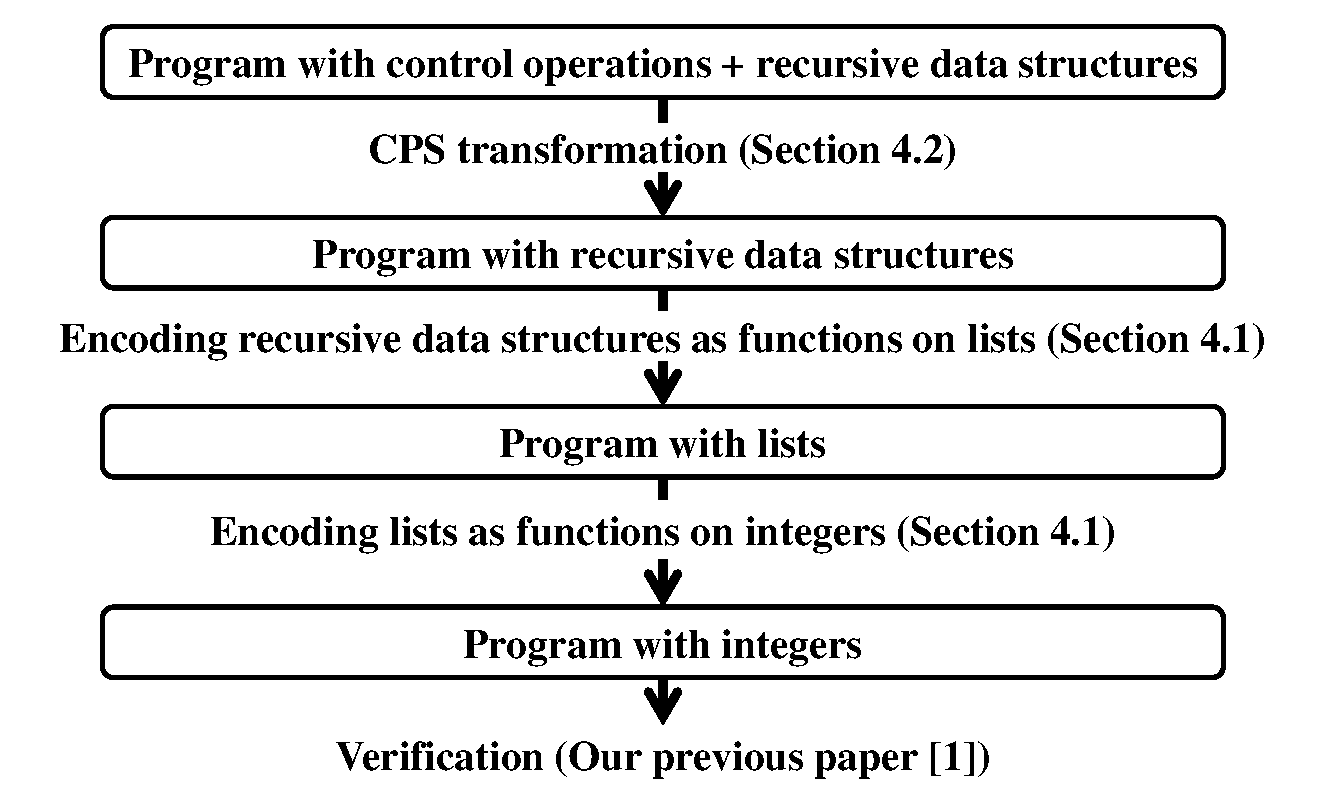
\includegraphics[scale=0.4]{extension.eps}
 \end{center}
\caption{The verification framework for recursive data structures and control operators}
\label{fig:extension}
\end{figure}



\subsection{Functional Encoding of Recursive Data Structures}
\label{sec:recdata}

In this section, we first formalize the encoding of lists, and then we discuss the
extension for user-defined recursive data structures.

%\[
%\begin{array}{lrl}
%D\text{ (programs)} &::=& \{f_1 = v_1, \dots, f_n = v_n\} \\
%t\text{ (terms)}
%  &::=& n \mid x \mid \Abs{x}{t} \mid t_1\ t_2 \mid \Op{v_1,\dots,v_n} \mid \If{t_1}{t_2}{t_3} \\
% &\mid& \FAIL \mid \Pair{v_1}{v_2} \mid \Fst{t} \mid \Snd{t} \mid \NIL \mid \Cons{v_1}{v_2} \\
% &\mid& (\MATCH\ {t_1}\ \WITH\ \NIL \ra {t_2} \mid \Cons{x_1}{x_2} \ra {t_3}) \\
%
%v\text{ (values)}
%  &::=& n \mid \Abs{x}{t} \mid \Pair{v_1}{v_2} \mid \NIL \mid \Cons{v_1}{v_2} \\
%
%E\text{ (eval. ctx.)}
%  &::=& [\,] \mid E\ t \mid \App{\Abs{x}{t}}{E} \mid \If{E}{t_2}{t_3} \mid \Fst{E} \mid \Snd{E} \\
% &\mid& (\Match{E}{t_2}{t_3}) \\
%
%\tau\text{ (types)} &::=& \INT \mid \TFun{\tau_1}{\tau_2} \mid \TPair{\tau_1}{\tau_2} \mid \List{\tau} \\
%\end{array}
%\]

%\begin{figure}[t]
%\begin{minipage}{\widthcoef\textwidth}
%\[
%\begin{array}{lrl}
%D\text{ (programs)} &::=& \{f_1 = v_1, \dots, f_n = v_n\} \\
%t\text{ (terms)}
%  &::=& n \mid x \mid \Abs{x}{t} \mid t_1\ t_2 \mid \Op{v_1,\dots,v_n} \mid \If{t_1}{t_2}{t_3} \\
% &\mid& \FAIL \mid \Pair{v_1}{v_2} \mid \Fst{t} \mid \Snd{t} \mid \NIL \mid \Cons{v_1}{v_2} \\
% &\mid& (\MATCH\ {t_1}\ \WITH\ \NIL \ra {t_2} \mid \Cons{x_1}{x_2} \ra {t_3}) \\
%
%v\text{ (values)}
%  &::=& n \mid \Abs{x}{t} \mid \Pair{v_1}{v_2} \mid \NIL \mid \Cons{v_1}{v_2} \\
%
%E\text{ (eval. ctx.)}
%  &::=& [\,] \mid E\ t \mid \App{\Abs{x}{t}}{E} \mid \If{E}{t_2}{t_3} \mid \Fst{E} \mid \Snd{E} \\
% &\mid& (\Match{E}{t_2}{t_3}) \\
%
%\tau\text{ (types)} &::=& \INT \mid \TFun{\tau_1}{\tau_2} \mid \TPair{\tau_1}{\tau_2} \mid \List{\tau} \\
%\end{array}
%\]
%\end{minipage}
%\caption{The syntax of source language with list}
%\label{fig:list-syntax}
%\end{figure}

\subsubsection{Functional Encoding of Lists}
\label{sec:list}

The idea is to encode a list into a pair of its length and a function that
maps indices to the elements of the list.  For example, the list
$[2;3;5]$ is encoded into the pair $(3,f)$ where $f(0) = 2$, $f(1) = 3$, and
$f(2) = 5$.  The primitive operations \texttt{nil}, \texttt{cons},
\texttt{is\_nil}, \texttt{head}, and \texttt{tail} for lists are defined
as follows.
\begin{alltt}
let nil = (0, fun _ -> fail)
let cons x (len,f) =
  let f' i = if i = 0 then x else f (i-1) in (len+1, f')
let is_nil (len,f) = len = 0
let head (len,f) = if is_nil (len,f) then fail else f 0
let tail (len,f) =
  (if is_nil (len,f) then fail else len-1), fun i -> f (i+1)
\end{alltt}
\texttt{nil} is translated into the pair of length $0$ and the
function that always fails.  \texttt{cons x xs} is translated into the
pair of its length and the function $\{0 \mapsto \mathtt{x}\} \cup \{i \mapsto
f (i-1) \mid i \neq 0\}$ where $f$ is the function part of encoding of
\texttt{xs}.  \texttt{is\_nil} just checks whether \texttt{len} is 0 or not.
\texttt{head} returns \texttt{f(0)}, i.e. the first
element of the list.  \texttt{tail} returns the pair of
\texttt{(len-1,f')} where $\texttt{f'(i)} = \texttt{f(i+1)}$.

%Since \texttt{f(i)} is the element whose position is \texttt{i} in the
%list, the encoded \texttt{head} returns \texttt{f(0)}, i.e. the $0$-th
%element of the list.  Function \texttt{tail} returns a pair of
%\texttt{(len-1,f')} where $\mathtt{f'(0)} = \mathtt{f(1)}$,
%$\mathtt{f'(1)} = \mathtt{f(2)}$, $\dots$

%Since the original \texttt{head} returns the head of a list,
%the encoded \texttt{head} returns the value

%consider the following
%program.
%\begin{alltt}
%let rec for_all p xs =
%  match xs with [] -> true
%          | x::xs' -> p x && for_all p xs'
%\end{alltt}
%\texttt{for\us{}all p [a1;...;an]} returns a boolean which represents
%whether \texttt{p(a$i$)} holds for every $i$.  We can obtain the
%following list-free program by the encoding mentioned above.
%\begin{alltt}
%let rec for_all p (len,f) =
%  if len = 0 then true
%  else let x = f 0 in
%       let len' = len - 1 in
%       let f' = fun i -> f (i+1) in
%         p x && for_all p (len',f')
%\end{alltt}
%The argument \texttt{xs} is translated into the pair of the length
%\texttt{len} and the function \texttt{f} such that \texttt{f($i$)}
%represents $i$-th element of the list \texttt{xs} (index is 1-origin.)
%The function \texttt{for\us{}all p}, which takes a list, is encoded to a
%higher-order function.  By this encoding, properties of lists are
%translated to ones of functions. For example, a property that
%\texttt{for\us{}all p xs} returns true, i.e. all the elements of
%\texttt{xs} satisfy \texttt{p}, is translated to a property that
%\texttt{f} always returns a positive integer.

This approach has the following advantages.  First, by encoding lists
into functions over integers, we can reuse the predicate
abstraction/discovery for integers.  Second, the encoding induces a
natural predicate abstraction of lists, which is general enough to
subsume various abstractions known in the literature, such as Dillig et
al.'s container abstraction~\cite{Dillig2011}.  In their abstraction
method for aggregate data structures like lists, a list is represented
as $\set{(v_1,P_1), \dots, (v_n,P_n)}$, a finite set of pairs of a
element of list and a condition for the index of the element.  For
example, $\set{(0,\TRUE)}$ denotes that all the elements are $0$ and
$\set{(1,\Abs{i}{i \mathop{\mathtt{mod}} 2 = 0})}$ denotes that the even
indexed elements are $1$.  On the other hand, by encoding a list as a
function, the same information can be represented as a refinement type
$\TFun{(i\COL\INT)}{\set{x\COL\INT\mid (P_1(i) \to x=v_1) \wedge \dots
\wedge (P_n(i) \to x=v_n)}}$.  For example, $\set{(1,\Abs{i}{i
\mathop{\mathtt{mod}} 2 = 0})}$ is represented as
$\TFun{(i\COL\INT)}{\set{x\COL\INT\mid i \mathop{\mathtt{mod}} 2 = 0 \to x=1}}$.  Moreover, our
approach can deal with list properties like ``the $i$-th
element of a list is greater than $i$,'' which cannot be represented by
the container abstraction.  Thus, our method, i.e., a combination of the encoding
and the predicate abstraction for integers, is strictly more powerful
than the container abstraction.

%\paragraph{Comparison with Dillig et al.'s appoach.}
%Dillig et al.~\cite{Dillig2011} have proposed an automatic technique for
%static reasoning about containers (e.g., maps, lists, and vectors). They
%model containers as functions that map a key to an abstract index that
%is mapped to a value corresponds to the index.  For example, a store
%includes list $[2;3]$ is abstracted as a map $\{\beta \mapsto
%\set{(\AbstLoc{\eta}{i}, \TRUE)}, \AbstLoc{\eta}{i} \mapsto
%\set{(2,i=0),(3,i=1),(\NIL,i \neq 0 \land i \neq 1)}\}$, where $\beta$
%is the memory location that stores the list, and $\AbstLoc{\eta}{i}$ is
%the abstract location indexed with $i$ that represents the list.  In the
%abstract store, $x \mapsto \set{(\pi_1, P_1), \dots, (\pi_n, P_n)}$
%represents that $x$ could have a value $\pi_i$ when $P_i$ holds.  Our
%approach is a generalization of their approach in the following sense:
%\begin{enumerate}
% \item While our abstraction uses arbitrary predicates for container elements,
%       they abstracts container elements to the set of unknown values,
%       integer constants, and locations.
% \item While our abstraction can depend on the index by the form ``if $P_(i)$
%       then $Q(i,v)$'' where $i$ is an index and $v$ is the element at the
%       index $i$, their abstraction can depend on the index only by the form ``if $P_(i)$
%       then $Q(v)$''.
%\end{enumerate}

%Once a target program is translated to a list-free program,
%we can apply our previous verification framework for higher-order programs with integers.

%Figure~\ref{fig:list-translation} shows the definition of the
%translation $\Trans{-}$.  Let $t$ be a list of the form
%$[v_0,\dots,v_{n-1}]$. $\Trans{t}$ denotes the pair of the length $n$ of
%$t$ and the function $\{0 \mapsto v_0, \dots, n-1 \mapsto v_{n-1}\}$
%that maps indices to elements of $t$.  $\NIL$ is translated into the pair of length $0$ and the
%function that always fails.  $\Cons{v_1}{v_2}$ is translated into the
%pair of its length and the function $\{0 \mapsto v_1\} \cup \{i \mapsto
%f (i-1) \mid i \neq 0\}$ where $f$ is the function part of encoding of
%$v_2$.  A pattern match is translated into an if-expression whose
%then-case and else-case respectively correspond to the $\NIL$ and
%$\Cons{x_1}{x_2}$ cases.
%
%\begin{figure}[t]
%\begin{minipage}{\widthcoef\textwidth}
%\[
%\begin{array}{l}
%% \Trans{n} = n \\
%% \Trans{x} = x \\
%% \Trans{\Fix{f}{x}{t}} = \Fix{f}{x}{\Trans{t}} \\
%% \Trans{t_1\ t_2} = \Trans{t_1}\ \Trans{t_2} \\
%% \Trans{\Op{v_1,\dots,v_n}} = \Op{\Trans{v_1}, \dots, \Trans{v_n}} \\
%% \Trans{\If{t_1}{t_2}{t_3}} = \If{\Trans{t_1}}{\Trans{t_2}}{\Trans{t_3}} \\
%% \Trans{\FAIL} = \FAIL \\
%% \Trans{\Pair{t_1}{t_2}} = \Pair{\Trans{t_1}}{\Trans{t_2}} \\
% \Trans{\NIL} = \Pair{0}{\Abs{u}{\FAIL}} \quad (\text{$u$ is fresh}) \\
%
% \Trans{\Cons{v_1}{v_2}} = (\Fst{v_2} + 1, \\
% \qquad \Abs{i}{\If{i-1}{\Trans{v_1}}{\Snd{v_2}\ (i-1)}}) \\
% \quad (\text{$i$ is fresh}) \\
%
% \Trans{\Match{t_1}{t_2}{t_3}} = \\
% \quad \Let{x}{\Trans{t_1}}{} \\
% \quad \Let{len}{\Fst{x}}{} \\
% \quad \Let{f}{\Snd{x}}{} \\
% \qquad \IF\ len\ \THEN\ \Trans{t_2} \\
% \qquad \ELSE\ \Let{x_1}{f\ 0}{}\\
% \qquad\qquad\, \Let{x_2}{\Pair{len - 1}{\Abs{i}{f (i+1)}}}{} \\
% \qquad\qquad\quad \Trans{t_3} \\
% \quad (\text{$x$, $len$, $f$ and $i$ are fresh}) \\
%\end{array}
%\]
%\end{minipage}
%\caption{Encoding of list (excerpt).}
%\label{fig:list-translation}
%\end{figure}

%The theorem below states that the translation $\Trans{-}$ is correct in
%the sense that if a source program fails, so does the translated program, and vice versa.
%\begin{theorem}[Correctness of translation]
%  \label{th:translation-list-correct}
%  Let $t$ be a term in a program $D$.
%  $t \Reds{D} \FAIL$ if and only if $\Trans{t} \Reds{D} \FAIL$.
%\end{theorem}



\subsubsection{Extension for Recursive Data Structures}
We discuss how to encode other recursive data structures.  We
translate programs with recursive data structures into programs with
lists by encoding recursive data structures to functions which map paths
of nodes to labels.  Here, a path and a label are represented as a list
of integers and an integer respectively.  For example, consider binary trees defined
as follows.
\begin{alltt}
type btree = Leaf | Node of btree * btree
\end{alltt}
A binary tree is encoded into a term of the type
$\TFun{\List\INT}{\INT}$.  For example, a binary tree
$\Node{\LEAF}{\Node{\LEAF}{\LEAF}}$ is encoded into a function $\{[]
\mapsto \NODE, [1] \mapsto \LEAF, [2] \mapsto \NODE, [2,1] \mapsto
\LEAF, [2,2] \mapsto \LEAF\}$ where $\LEAF$ and $\NODE$ are defined as
some integers.
Here is another example, the encoding of a pattern matching.
\begin{alltt}
match x with Constr_1(x1, x2, ...) -> t | Constr_2(...) -> ...
\end{alltt}
The expression above is encoded to the following expression.
\begin{alltt}
let Constr_1 = 1 in ... let Constr_n = n in
  match x nil with Constr_1 -> let x1 xs = x (cons 1 xs) in ...
                               let xn xs = x (cons n xs) in t'
                 | Constr_2 -> ...
\end{alltt}
Here, \texttt{t'} is the encoding of \texttt{t}. The pattern matching in
trees is translated to the pattern matching in labels, represented as
integers.  A subterm of a tree is obtained by adding the index to the head of the path.
%\begin{alltt}
%let rec get_child t =
%  match t with
%    Constr(t1,t2)Leaf -> fail
%  | Node(t1,t2) -> (t1, t2)
%\end{alltt}
%This program takes an unlabeled binary tree and returns its children.
%The program is translated into the following program with no recursive
%data structures except lists.
%\begin{alltt}
%let Leaf = 0
%let Node = 1
%let rec get_child t =
%  match t nil with
%    Leaf -> fail
%  | Node ->
%      let t1 xs = t (cons 0 xs) in
%      let t2 xs = t (cons 1 xs) in
%        (t1, t2)
%\end{alltt}

We treat only regular algebraic data types, i.e., the combination of sum
types and product types, which cannot have function types as arguments
of constructors.  Types of recursive data structures are represented as
recursive types.  We require that in a recursive type
$\RecType{\alpha}{\tau}$, $\alpha$ does not occur below function type
constructors. For example, $\List{\TFun{\INT}{\INT}}$ is OK, but neither
$\RecType{\alpha}{\TFun{\alpha}{\INT}}$ nor
$\RecType{\alpha}{\TFun{\INT}{\alpha}}$ is allowed.

%The reason is that the encoding recursive data types generates recursive types again.

%We introduce the language extended with recursive data structures.
%Figure~\ref{fig:rec-syntax} shows the syntax of the language.  The
%meta-variable $\CONSTR$ ranges over the sets of constructor names.
%$\Constr{}{v_1,\dots,v_k}$ is a constructor and $\MatchRec{t}{t_1}{t_k}$
%is a destructor for a type
%$\Constr{1}{\widetilde{\phi_1}} + \ldots + \Constr{k}{\widetilde{\phi_k}}$.
%A program is a pair of function definitions and type definitions
%$\gamma_1=\rho_1, \dots, \gamma_m=\rho_m$.
%A type definition
%$\gamma_1=\Constr{1}{\widetilde{\phi_1}} + \dots + \Constr{k}{\widetilde{\phi_k}}$
%means that type $\gamma$ has
%constructors $\CONSTR_1, \dots, \CONSTR_k$ and the types of the
%arguments of $C_i$ are $\widetilde{\phi_i}$.
%Note that, expressions for pattern matching on lists are distinct
%from ones for pattern matching on recursive data structures.  We restrict the types of the
%constructor arguments, represented by meta-variable $\phi$, to
%$\INT$ or recursive data types for the sake of simplicity.
%
%%We assume that $\gamma$ and $\CONSTR$ are distinct from others.
%
%
%\begin{figure}[t]
%\begin{minipage}{\textwidth}
%\[
%\begin{array}{lrl}
%D\text{ (program)} &::=& \{ f_1=t_1, \dots, f_n=t_n; \gamma_1=\rho_1, \ldots, \gamma_m=\rho_m \} \\
%t\text{ (terms)} &::=& \ldots \mid \Constr{}{\widetilde{v}} \mid (\MatchRec{t}{t_1}{t_k}) \\
%
%\rho\text{ (rec. type)} &::=& \Constr{1}{\widetilde{\phi_1}} + \dots + \Constr{k}{\widetilde{\phi_k}} \\
%\phi &::=& \INT \mid \gamma \\
%\tau\text{ (types)} &::=& \ldots \mid \gamma \\
%\end{array}
%\]
%\end{minipage}
%\caption{The syntax of language extended with recursive data structures}
%\label{fig:rec-syntax}
%\end{figure}
%
%\begin{example}
%A type definition for rose trees is represented as the following.
%\begin{eqnarray*}
% \RTREE &=& \RTNODE(\RTLIST) \\
% \RTLIST &=& \RTNIL() + \RTCONS(\RTREE, \RTLIST)
%\end{eqnarray*}
%%\memo{$\TREE = \NIL() + \NODE(\TREE, \TREE)$}
%\end{example}
%
%
%Figure~\ref{fig:rec-translation} shows the definitions of the translation $\TransRec{D}{-}$.
%$\TransRec{D}{t}$ denotes a function that maps paths to nodes of $t$.
%%Translation of constructors and destructors of lists are trivial, translate recursively.
%%We translate a recursive data $\Constr{}{v_1,\dots,v_n}$ into a function
%%that returns
%$\TransRec{D}{\Constr{}{v_1,\dots,v_n}}$ is a function that returns
%\begin{itemize}
% \item an integer $\TransRec{D}{C}$, correspondence number to $\CONSTR$, for $\NIL$,
% \item $v_k$ for a list whose head is $k$ when $v_k$ has type $\INT$, and
% \item $\App{\TransRec{D}{v_k}}{p}$ for a list that has the form of
%       $\Cons{k}{p}$ when $v_k$ has a recursive data type.
%\end{itemize}
%We translate $\MatchRec{t}{t_1}{t_k}$ into a if-expression that
%checks what is $\App{\TransRec{D}{t}}{\NIL}$, the root node label of
%$t$.  We can obtain the translated value%, the constructor
%argument, to which it bound to variable $x_{ij}$ by
%$\App{f}{(\Cons{i}{\NIL})}$ for $\INT$ and
%$\Abs{p}{\App{f}{(\Cons{i}{p})}}$ for recursive data types.
%%\TODO{add (or rewrite to) more intuitionistic explanation}




%\begin{figure}[t]
%\begin{minipage}{\textwidth}
%\[
%\begin{array}{l}
%% \TransRec{D}{n} = n \\
%% \TransRec{D}{x} = x \\
%% \TransRec{D}{\Fix{f}{x}{t}} = \Fix{f}{x}{\TransRec{D}{t}} \\
%% \TransRec{D}{t_1\ t_2} = \TransRec{D}{t_1}\ \TransRec{D}{t_2} \\
%% \TransRec{D}{\Op{t_1,\dots,t_n}} = \Op{\TransRec{D}{t_1}, \dots, \TransRec{D}{t_n}} \\
%% \TransRec{D}{\If{t_1}{t_2}{t_3}} = \If{\TransRec{D}{t_1}}{\TransRec{D}{t_2}}{\TransRec{D}{t_3}} \\
%% \TransRec{D}{\FAIL} = \FAIL \\
%% \TransRec{D}{\Pair{t_1}{t_2}} = \Pair{\TransRec{D}{t_1}}{\TransRec{D}{t_2}} \\
% \TransRec{D}{\NIL} = \NIL \\
% \TransRec{D}{\Cons{t_1}{t_2}} = \Cons{\TransRec{D}{t_1}}{\TransRec{D}{t_2}} \\
% \TransRec{D}{\Match{t_1}{t_2}{t_3}} = \\
%  \quad \Match{\TransRec{D}{t_1}}{\TransRec{D}{t_2}}{\TransRec{D}{t_3}} \\
%
% \TransRec{D}{\Constr{}{v_1,\dots,v_n}} = \\\qquad
%  \Abs{x}{}\MATCH\ x\ \WITH\ \NIL \ra \TransRec{D}{\CONSTR} \\\qquad\qquad
%  \begin{array}{ll}
%   \mid \Cons{k}{p} \ra & \If{k - 1}{\RecConstr{D}{C}{1}{p}{\TransRec{D}{v_1}}}{} \\
%                        & \If{k - 2}{\RecConstr{D}{C}{2}{p}{\TransRec{D}{v_2}}}{} \\
%                        & \quad \dots \\
%                        & \If{k - n}{\RecConstr{D}{C}{n}{p}{\TransRec{D}{v_n}}}{\FAIL} \\
%  \end{array} \\
% \TransRec{D}{\MatchRec{t}{t_1}{t_k}} = \\
% \quad \Let{f}{\TransRec{D}{t}}{} \\
% \quad \Let{l}{\App{f}{\NIL}}{} \\
% \qquad \If{l - 1}{\RecDestr{D}{\CONSTR_1}{f}{\TransRec{D}{t_1}}}{} \\
% \qquad \If{l - 2}{\RecDestr{D}{\CONSTR_2}{f}{\TransRec{D}{t_2}}}{} \\
% \qquad \quad \dots \\
% \qquad \If{l - k}{\RecDestr{D}{\CONSTR_k}{f}{\TransRec{D}{t_k}}}{\FAIL} \\
%\end{array}
%\]
%\[
%\begin{array}{l}
% \RecConstr{D}{\CONSTR}{k}{p}{v} =
%  \left\{
%  \begin{array}{ll}
%    v          & \quad \text{($\phi_k = \INT$)} \\
%    \App{v}{p} & \quad \text{(otherwise)}
%  \end{array}
%  \right. \\
%\qquad \text{where $D \ni (\gamma = \cdots + \Constr{}{\phi_1,\dots,\phi_j,\dots,\phi_n} + \cdots)$}
%
%%%% \begin{array}{rl}
%%%%   \RecDestr{D}{\gamma_i}{f}{j}{t} =
%%%%     & \Let{x_1}{\Abs{p}{f\ (\Cons{1}{p})}}{} \\
%%%%     & \dots \\
%%%%     & \Let{x_{n_i}}{\Abs{p}{f\ (\Cons{n_i}{p})}}{t}
%%%% \end{array} \\
%\end{array}
%\]
%
%\[
%\begin{array}{l}
% \begin{array}{rl}
%   \RecDestr{D}{\CONSTR}{f}{t} =
%     & \Let{x_1}{\RecDestrBase{D}{\CONSTR}{f}{1}}{} \\
%     & \quad \dots \\
%     & \Let{x_n}{\RecDestrBase{D}{\CONSTR}{f}{n}}{t}
% \end{array} \\
% \RecDestrBase{D}{\CONSTR}{f}{i} =
%  \left\{
%  \begin{array}{ll}
%    \App{f}{(\Cons{i}{\NIL})}       & \quad \text{($\phi_i = \INT$)} \\
%    \Abs{p}{\App{f}{(\Cons{i}{p})}} & \quad \text{(otherwise)}
%  \end{array}
%  \right. \\
%\qquad \text{where $D \ni (\gamma = \cdots + \Constr{}{\phi_1,\dots,\phi_i,\dots,\phi_n} + \cdots)$}
% \end{array}
%\]
%\end{minipage}
%\caption{Encoding of recursive data structures.
%$\TransRec{D}{\CONSTR}$ is an unique integer corresponds to $\CONSTR$.}
%\label{fig:rec-translation}
%\end{figure}


\subsection{Extension for Control Operations}
\label{sec:control} We can extend the framework to deal with control
operations (e.g., exceptions and \texttt{call/cc}) by removing these
from a program by CPS transformation~\cite{Nielsen2001}.

%Consider the following program (written in OCaml style).
The following program calculates factorial and raise an exception if
a negative number or zero is given.
\begin{alltt}
exception NotPositive
let rec fact n =
  if n <= 0 then raise NotPositive
  else try n * fact (n - 1) exn with NotPositive -> 1
let main n = try fact n with NotPositive -> assert (n <= 0); 0
\end{alltt}
We can translate this program to an exception-free program by CPS transformation.
The following is the result of CPS transformation.
\begin{alltt}
type exc = NotPositive
let rec fact n k exn =
  if n <= 0 then exn NotPositive
  else let exn' e = match e with NotPositive -> k 1 in
         fact (n - 1) (fun r -> k (n * r))) exn'
let main n k =
  fact n k (fun e -> match e with NotPositive -> assert (n <= 0); k 0
                                | _ -> assert false)
\end{alltt}
Once the exception is removed, we can apply our verification method to the
program.



\section{Implementation and Preliminary Experiments}
\label{sec:experiments}

To evaluate the extended framework, we have implemented a prototype
verifier for higher-order programs with lists and exceptions.
%The verifier takes an OCaml program as input.
Our verifier uses TRecS~\cite{KobayashiPOPL2009,KobayashiPPDP2009} as
the underlying higher-order model checker (for Step 3 in
Fig.~\ref{fig:overview}), and uses CSIsat~\cite{Beyer2008} for predicate
discovery (for Step 5).  CVC3~\cite{Barrett2007} is used for unsafety
check (for Step 4) and predicate abstraction (for Step 1).

Table~\ref{tbl:exp} shows the results of the experiments.
The column ``size'' shows the word counts of the program.
The last column shows the number of CEGAR-cycle and the running time measured.
The programs are safe, and have been verified correctly.


\begin{table}
\caption{Results of preliminary experiments}
\label{tbl:exp}
\begin{center}
\begin{tabular}{|l|r|r|r|r|r|r|r|}
\hline
            &       &       &                      & \multicolumn{4}{|c|}{cycle, time [sec]} \\
\cline{5-8}
program & size & order & \# of pred. in annot. & \cc{no opt.} & \cc{CPS} & \cc{Abst.} & \cc{both} \\
\hline
fold\_right      &  64 & 2 & 0 & 5, 8.53 & 5, 20.9 & 2, 0.36 & 2, 0.19 \\
forall\_eq\_pair &  55 & 1 & 0 & 4, 2.32 & 4, 0.94 & 1, 0.76 & 1, 0.23 \\
forall\_leq      &  55 & 2 & 0 & 4, 2.10 & 4, 0.86 & 1, 0.17 & 1, 0.14 \\
isnil            &  52 & 1 & 0 & 3, 0.16 & 3, 0.15 & 2, 0.12 & 2, 0.12 \\
iter             &  59 & 2 & 0 & 4, 1.60 & 4, 0.62 & 1, 0.16 & 1, 0.11 \\
%length3          &  50 & 1 & 0 &       - &       - &       - & -, -    \\
mem              &  74 & 1 & 0 & 4, 1.05 & 4, 0.34 & 3, 0.41 & 3, 0.17 \\
nth0             &  78 & 1 & 0 & 3, 0.26 & 3, 0.16 & 3, 0.25 & 3, 0.17 \\
harmonic         & 101 & 2 & 0 &       - & 5, 1.77 & 1, 0.16 & 1, 0.09 \\
fold\_left       &  64 & 2 & 0 &       - &       - &       - & 2, 0.23 \\
%iter\_fun\_list  &  59 & 3 & 0 &       - &       - &       - & -, -    \\
zip              &  69 & 1 & 0 &       - &       - &       - & 2, 0.11 \\
%map              &  85 & 2 & 0 &       - &       - &       - & -, -    \\
%\hline
inits            & 111 & 2 & 0 &       - &       - & 2, 2.53 & 3, 1.06 \\
risers           &  79 & 1 & 0 &       - &       - & 4, 2.72 & 4, 1.17 \\
%ground  &   - & - & - & - & - & - & - & - & - \\
\hline
\end{tabular}
\end{center}
\end{table}

The applications of two optimized techniques enable verification of the
programs ``harmonic'', ``fold\_left'', ``zip'', ``inits'', and ``risers'', and reduce the
running time.  Especially, the application of selective CPS
transformation reduces the running time, and selective predicate
abstraction reduces the number of CEGAR cycles.

The details of the programs are showed as follows.
\begin{itemize}
%\item ``fold\_right'' defines 
\item ``forall\_eq\_pair'' defines a generator of lists of the form
      $[(n_1,n_1);\dots;(n_k,n_k)]$, and function \texttt{forall} that
      takes a predicate $p$ as a function and a list and checks if all
      elements of the list satisfy the $p$.
\item ``forall\_leq'' defines a generator of positive integer lists and
      the function \texttt{forall}.
\item ``isnil'' defines a generator of integer lists and a function that
      takes a list and checks whether the list is nil or not.
\item ``iter'' defines a generator of positive integer lists and the
      function \texttt{iter}.
\item ``mem'' defines a generator of lists consists of the same elements
      and function \texttt{mem} that takes a value and a list, then
      checks the value is in the list.
\item ``nth0'' defines a generator of integer lists and function
      ``nth'' that takes an index $i$ and a list and returns $i$-th element of the list.
\item ``harmonic'' defines a function that calculates $\sum_{1 \leq k}
      \frac{n}{k}$ for some $n$, $k$ using a fold function for lists.
      The program asserts that a zero division cannot occurs.
\item ``fold\_left'' defines a fold function for lists and sum
\item ``zip''
\item ``inits''
\item ``risers''
\end{itemize}

%\begin{itemize}
%\item fold\_right
%\begin{alltt}
%let rec fold_right (f:int->int->int) xs acc =
%  match xs with
%    [] -> acc
%  | x::xs' -> f x (fold_right f xs' acc)
%
%let rec make_list n =
%  if n < 0
%  then []
%  else n :: make_list (n-1)
%
%let add x y = x + y
%
%let main n m =
%  let xs = make_list n in
%    assert (fold_right add xs m >= m)
%\end{alltt}
%
%\item forall\_eq\_pair
%\begin{alltt}
%let rec for_all f (xs:(int*int) list) =
%  match xs with
%      [] -> true
%    | x::xs' ->
%        f x && for_all f xs'
%
%let rec eq_pair ((x:int),(y:int)) = x = y
%
%let rec make_list n =
%  if n < 0
%  then []
%  else (n,n) :: make_list (n-1)
%
%let main n = assert (for_all eq_pair (make_list n))
%\end{alltt}
%
%\item forall\_leq
%\begin{alltt}
%let rec for_all f (xs:int list) =
%  match xs with
%      [] -> true
%    | x::xs' ->
%        f x && for_all f xs'
%
%let rec check x = x >= 0
%
%let rec make_list n =
%  if n < 0
%  then []
%  else n :: make_list (n-1)
%
%let main n = assert (for_all check (make_list n))
%\end{alltt}
%
%\item isnil
%\begin{alltt}
%let is_nil (xs:int list) =
%  match xs with
%      [] -> true
%    | _ -> false
%
%let rec make_list n =
%  if n = 0
%  then []
%  else n :: make_list (n-1)
%
%let main n =
%  let xs = make_list n in
%    if n > 0
%    then assert (not (is_nil xs))
%    else ()
%\end{alltt}
%
%\item iter
%\begin{alltt}
%let rec iter (f:int -> unit) xs =
%  match xs with
%      [] -> ()
%    | x::xs' -> f x; iter f xs'
%
%let rec make_list n =
%  if n < 0
%  then []
%  else n :: make_list (n-1)
%
%let check x = assert (x >= 0)
%
%let main n =
%  let xs = make_list n in
%    iter check xs
%\end{alltt}
%
%\item length3
%\begin{alltt}
%let rec length (xs:int list) =
%  match xs with
%      [] -> 0
%    | _::xs' -> 1 + length xs'
%
%let rec make_list n =
%  if n = 0
%  then []
%  else n :: make_list (n-1)
%
%let main n =
%  let xs = make_list n in
%    assert (length xs = n)
%\end{alltt}
%
%\item mem
%\begin{alltt}
%let rec mem (x:int) xs =
%  match xs with
%      [] -> false
%    | x'::xs -> x = x' || mem x xs
%
%let rec make_list n (x:int) =
%  if n < 0
%  then []
%  else x :: make_list (n-1) x
%
%let is_nil (xs:int list) =
%  match xs with
%      [] -> true
%    | _ -> false
%
%let main n m =
%  let xs = make_list n m in
%    assert (is_nil xs || mem m xs)
%\end{alltt}
%
%\item nth0
%\begin{alltt}
%let is_nil (xs:int list) =
%  match xs with
%      [] -> true
%    | _ -> false
%
%let rec nth n (xs:int list) =
%  match xs with
%    | [] -> assert false
%    | x::xs' -> if n = 0 then x else nth (n-1) xs'
%
%let rec make_list n =
%  if n < 0
%  then []
%  else n :: make_list (n-1)
%
%let main n =
%  let xs = make_list n in
%    if is_nil xs
%    then 0
%    else nth 0 xs
%\end{alltt}
%
%\item harmonic
%\begin{alltt}
%let rec div x y =
%  assert (y <> 0);
%  if x < y
%  then 0
%  else 1 + div (x-y) y
%
%let rec fold_left (f:int->int->int) acc xs =
%  match xs with
%      [] -> acc
%    | x::xs' -> fold_left f (f acc x) xs'
%
%let rec range i j =
%  if i > j then
%    []
%  else
%    let is = range (i+1) j in
%      i::is
%
%let harmonic n =
%  let ds = range 1 n in
%    fold_left (fun s k -> s + div 10000 k) 0 ds
%\end{alltt}
%
%\item fold\_left
%\begin{alltt}
%let rec fold_left (f:int->int->int) acc xs =
%  match xs with
%      [] -> acc
%    | x::xs' -> fold_left f (f acc x) xs'
%
%let rec make_list n =
%  if n < 0
%  then []
%  else n :: make_list (n-1)
%
%let add x y = x + y
%
%let main n m =
%  let xs = make_list n in
%    assert (fold_left add m xs >= m)
%\end{alltt}
%
%\item iter\_fun\_list
%\begin{alltt}
%let rec iter (f:(int->unit)->unit) xs =
%  match xs with
%      [] -> ()
%    | x::xs' -> f x; iter f xs'
%
%let rec make_list n =
%  if n < 0
%  then []
%  else (fun x -> assert (n >= x)) :: make_list (n-1)
%
%let main n =
%  let xs = make_list n in
%    iter (fun f -> f 0) xs
%\end{alltt}
%
%
%\item map
%\begin{alltt}
%let rec map f xs =
%  match xs with
%      [] -> []
%    | x::xs' -> f x :: map f xs'
%
%let rec length xs =
%  match xs with
%      [] -> 0
%    | _::xs' -> 1 + length xs'
%
%let rec make_list n =
%  if n < 0
%  then []
%  else n :: make_list (n-1)
%
%let succ x = x + 1
%
%let main n =
%  let xs = make_list n in
%  let xs' = map succ xs in
%    assert (length xs = length xs')
%\end{alltt}
%
%\item zip
%\begin{alltt}
%let rec zip xs ys =
%  match xs with
%      [] ->
%        begin
%          match ys with
%              [] -> []
%            | _ -> assert false
%        end
%    | x::xs' ->
%        match ys with
%            [] -> assert false
%          | y::ys' -> (x,y)::zip xs' ys'
%
%let rec make_list n =
%  if n < 0
%  then []
%  else n :: make_list (n-1)
%
%let main n =
%  let xs = make_list n in
%    zip xs xs
%\end{alltt}
%
%\item inits
%\begin{alltt}
%let rec make_list m =
%  if m <= 0
%  then []
%  else Random.int 0 :: make_list (m-1)
%
%let rec make_list_list m =
%  if m <=0 
%  then []
%  else make_list (Random.int 0) :: make_list_list (m-1)
%
%let head = function
%    [] -> assert false
%  | x::xs -> x
%
%let ne = function
%    [] -> 0
%  | x::xs -> 1
%
%let rec filter p = function
%    [] -> []
%  | x::xs -> if p x = 1 then x::(filter p xs) else filter p xs
%
%let rec map f = function
%    [] -> []
%  | x::xs -> f x :: map f xs
%
%let main m = map head (filter ne (make_list_list m))
%\end{alltt}
%
%\end{itemize}



\section{Related Work}
\label{sec:related}

\subsection{Container Abstraction}
There are several
frameworks~\cite{Kawaguchi2009,Chin2003,Unno2010,Ong2011} that aimed at
verification of functional programs with data structures.

Ong et al.~have proposed the verification framework for recursion scheme with
recursive data structures, called Pattern Matching Recursion Scheme.  As stated in
Sect.~\ref{}, their framework requires control flow analysis. Moreover,
the framework cannot deal with some regular properties. For example, the
framework cannot verify that a list obtained by applying the following
``id'' function to an even length list is also even length.
\begin{alltt}
let rec id x = match x with nil -> nil | cons x xs -> cons x (id xs)
\end{alltt}

Unno et al.~have proposed the verification framework for higher-order
tree processing functional programs. Their framework distinguish that
input tree types and output tree types.  In order to use output trees of
some function as input trees to some function, programmers have to
insert coercion functions with annotations of the properties of input
trees and the properties of output trees.
%\cc{This is the heavy burden to programmers}

Kawaguchi et al.'s liquid type inferecne~\cite{Kawaguchi2009} are
semi-automated verification framework based on refinement types.  Their
framework requires the shape of predicates, called logical qualifiers,
to users.  The limitation of our framework is that it cannot deal with
\cc{recursive dependency} on recursive data structures such that
orderedness.  Their framework can deal with recursive dependent type
such that $\App{\INT}{\LIST_\leq} = \mu t.\NIL +
\Cons{x_1\COL\INT}{x_2\COL\App{\{\nu\COL\INT \mid \nu \leq
x_1\}}{\LIST}}$, i.e., ordered lists of integers.  The framework,
however, cannot deal with the properties of list elements related to its
indices like that the $i$-th element of a list is greater than $i$.

Dillig et al.~\cite{Dillig2011} have proposed an automatic technique for
static reasoning about containers.  The proposed framework is based on
an abstract interpretation for containers.  Their framework is similar
to our framework in the sense that they model containers as mappings
from location to values.  While they consider the client-side use of the
specific data structures (i.e. containers), we consider a more general
class of data structures include user-defined data structures.

Chin et al.'s sized type inference~\cite{Chin2003}.  Their framework
infers invariant of recursive functions by fix-point computation.  The
framework cannot handle higher-order functions.

%\subsection{}
%[Comparison with others (Soonho Kong et al. APLAS10, etc.)]

\section{Conclusion}
\label{sec:conclusion}

We have proposed extensions and refinements to realize a scalable
software model checker for higher-order programs.  The proposed method
is simple and general for verifications of higher-order programs.  We
have identified the problems of the previous verification method, and proposed
the optimization techniques to overcome the problems.  We have
implemented a prototype verifier for higher-order programs with lists,
which works well for several programs.  An implementation for general
recursive data structures and experiments are left for future work.




\vspace{-5pt}

\bibliographystyle{abbrvnat}
\bibliography{main,abbrv,prog_lang}

%\appendix

\section{Rules for Selective Predicate Abstraction}

\TODO{List all the rules for selective predicate abstraction.}
%This section shows all the rules for selective predicate abstraction.

\section{Proof of Theorem~\ref{thm:abst_sound}}

\TODO{Add explanation of the proof}
\memo{The only differences from PLDI are the proofs of Lemma~\ref{lem:sub} and Lemma~\ref{lem:sim}.
Other proof are irrelevant to \rn{AppExp}.}


\begin{lemma}
\label{lem:sim}
Suppose that
\begin{itemize}
\item $\Abst{\Gamma}{E}{e_1}{\sigma}{e_2}$ and
\item $e_1 \Redwith{l}{D_1} e_1'$.
\end{itemize}
There exists $e_2'$ such that:
\begin{itemize}
\item $\Abst{\Gamma}{E}{e_1'}{\sigma}{e_2'}$ and
\item $e_2 \Redswith{l}{D_2} e_2'$.
\end{itemize}
\end{lemma}

\begin{lemma}
\label{lem:const}
If $\Abst{\Gamma}{E}{c}{b[\seq{P}]}{e}$, then
$e \Redswith{\epsilon}{D_2} \Tuple{\seq{v}} \equiv \Tuple{\seq{P}(c)}$ for some $\seq{v}$.
\end{lemma}

\begin{lemma}
\label{lem:fail}
If $\Abst{\Gamma}{E}{\FAIL}{\sigma}{e}$, then $e
\Redswith{\epsilon}{D_2} \FAIL$.
\end{lemma}

\begin{lemma}
\label{lem:sub}
If $\Abst{\Gamma,\seq{x}_1:\seq{\sigma}_1}{E}{v}{\sigma'}{v'}$ and
$\Abst{\Gamma,\seq{x}_1:\seq{\sigma}_1,x:\sigma',\seq{x}_2:\seq{\sigma}_2}{E}{e}{\sigma}{e'}$, then
$\Abst{\Gamma,\seq{x}_1:\seq{\sigma}_1,\seq{x}_2:[v/x]\seq{\sigma}_2}{E}{[v/x]e}{[v/x]\sigma}{[v'/x]e'}$.
\end{lemma}

\begin{lemma}
\label{lem:subb}
Suppose that
\begin{itemize}
\item $\Abst{\Gamma,\Gamma'}{E}{e}{\sigma'}{e_1}$,
\item $\Abst{\Gamma,r:\sigma'}{E}{r}{\sigma}{e_2}$, and
%\item $\sigma,\sigma'$ are base types, and
\item $r \not\in \FV{\sigma}$.
\end{itemize}
We obtain $\Abst{\Gamma,\Gamma'}{E}{e}{\sigma}{\Let{r}{e_1}{e_2}}$.
\end{lemma}

\begin{lemma}
\label{lem:val}
If $\Abst{\Gamma}{E}{v}{\sigma}{e}$, then $\Abst{\Gamma}{E}{v}{\sigma}{v'}$ and
$e \Redswith{\epsilon}{} v'$ for some $v'$.
\end{lemma}

Lemma~\ref{lem:val} immediately follows from the following lemma:

\begin{lemma}
\label{lem:val_aux}
If $\Abst{\Gamma,x_1:\sigma_1,\dots,x_k:\sigma_k}{E}{v}{\sigma}{e}$ and
$\AbstT{\Gamma,x_1:\sigma_1,\dots,x_{i-1}:\sigma_{i-1}}{E}{v_i}{\sigma_i}{v_i'}$ for each $i \in \set{1,\dots,k}$, then
there exists some value $\theta_k v'$ such that:
\begin{itemize}
\item $\AbstT{\Gamma,x_1:\sigma_1,\dots,x_k:\sigma_k}{E}{v}{\sigma}{v'}$ and
\item $\theta_k e \equiv \theta_k v'$.
\end{itemize}
Here, $\theta_i$ represents $[v_1'/x_1]\cdots[v_i'/x_i]$, and we
write $\AbstT{\Gamma,x_1:\sigma_1,\dots,x_k:\sigma_k}{E}{v}{\sigma}{v'}$ if:
\begin{itemize}
\item $\Abst{\Gamma,x_1:\sigma_1,\dots,x_k:\sigma_k}{E}{v}{\sigma}{v'}$ and
\item if $\sigma=x_{k+1}:\sigma_{k+1} \to \sigma'$,
$\sigma'$ is a function type, and
$\AbstT{\Gamma,x_1:\sigma_1,\dots,x_k:\sigma_k}{E}{v_{k+1}}{\sigma_{k+1}}{v_{k+1}'}$, then
$\theta_{k+1} (v'\ x_{k+1}) \equiv \theta_{E}{k+1} v''$ and
$\AbstT{\Gamma,x_1:\sigma_1,\dots,x_{k+1}:\sigma_{k+1}}{E}{v\ x_{k+1}}{\sigma'}{v''}$
for some value $\theta_{k+1} v''$.
\end{itemize}
\end{lemma}

\begin{lemma}
\label{lem:coerce}
Suppose that
\begin{itemize}
\item $\Abst{\Gamma,r:(x:\sigma_1 \to \sigma_2)}{E}{r}{(x:\sigma_1' \to \sigma_2')}{e_r}$,
\item $\Abst{\Gamma}{E}{v_1}{\sigma_1 \to \sigma_2}{v_1'}$, and
\item $\Abst{\Gamma}{E}{v_2}{\sigma_1'}{v_2'}$.
\end{itemize}
There exist $e_r'$ and $v_2''$ such that:
\begin{itemize}
\item $(\Let{r}{v_1'}{e_r})\ v_2' \Redswith{\epsilon}{}\equiv \Let{r}{v_1'\ v_2''}e_r'$,
\item $\Abst{\Gamma,r:[v_1/x]\sigma_2}{E}{r}{[v_1/x]\sigma_2'}{e_r'}$, and
\item $\Abst{\Gamma}{E}{v_2}{\sigma_1}{v_2''}$.
\end{itemize}
\end{lemma}

\begin{lemma}
\label{lem:fun}
Suppose that
\begin{itemize}
\item $\Abst{\Gamma}{E}{f\ v_1\cdots v_j}{(x_{j+1}\COL\sigma_{j+1}' \to \cdots \to x_k\COL\sigma_k' \to b[\seq{Q}])}{e}$,
\item $j<k$,
\item $\Gamma(f)=x_1:\sigma_1 \to \cdots \to x_k:\sigma_k \to b[\seq{P}]$, and
\item $\Abst{\Gamma}{E}{v_{j+1}}{\sigma_{j+1}'}{v_{j+1}''}$.
\end{itemize}
There exist $e_r,v_1',\dots,v_{j+1}'$ such that:
\begin{itemize}
\item $e\ v_{j+1}'' \Redswith{\epsilon}{}\equiv \Let{r}{f\ v_1'\cdots v_{j+1}'}{e_r}$,
\item
$\Abst{\Gamma,r:[v_1/x_1,\dots,v_{j+1}/x_{j+1}](x_{j+2}:\sigma_{j+2} \to \cdots \to x_k:\sigma_k \to b[\seq{P}])}{E}
    {r}
    {[v_{j+1}/x_{j+1}](x_{j+2}\COL\sigma_{j+2}' \to \cdots \to x_k\COL\sigma_k' \to b[\seq{Q}])}
    {e_r}$, and
\item for each $i \in \set{1,\dots,j+1}$, $\Abst{\Gamma}{E}{v_i}{[v_1/x_1,\dots,v_{i-1}/x_{i-1}]\sigma_i}{v_i'}$.
\end{itemize}
\end{lemma}

\begin{proof}[Proof of Lemma~\ref{lem:sub}]
We prove the lemma by induction on the derivation of
$\Abst{\Gamma,\seq{x}_1:\seq{\sigma}_1,x:\sigma',\seq{x}_2:\seq{\sigma}_2}{E}{e}{\sigma}{e'}$.
We proceed by case analysis on the last rule used.
We only show the case $\rn{A-AppExp}$.
We have
\begin{itemize}
\item $e = \App{x'}{\seq{v}}$,
\item $E(x') = \Abs{x_1}{\cdots\Abs{x_n}{e''}}$,
\item $\Abst{\Gamma,\seq{x}_1:\seq{\sigma}_1,x:\sigma',\seq{x}_2:\seq{\sigma}_2}{E}{[v_1/x_1,\dots,v_n/x_n]e''}{\sigma}{e'}$.
\end{itemize}
By I.H., we get $\Abst{\Gamma,\seq{x}_1:\seq{\sigma}_1,\seq{x}_2:[v/x]\seq{\sigma}_2}{E}{[v/x][v_1/x_1,\dots,v_n/x_n]e''}{[v/x]\sigma}{[v'/x]e'}$.
By \rn{A-AppExp}, we obtain $\Abst{\Gamma,\seq{x}_1:\seq{\sigma}_1,\seq{x}_2:[v/x]\seq{\sigma}_2}{E}{[v/x]e}{[v/x]\sigma}{[v'/x]e'}$.
\qed
\end{proof}

Now, we are ready to prove that each reduction $\Redwith{l}{D_1}$ can be simulated by $\Redswith{l}{D_2}$.

\begin{proof}[Proof of Lemma~\ref{lem:sim}]
We prove the lemma by induction on the derivation of $\Abst{\Gamma}{E}{e_1}{\sigma}{e_2}$.
We proceed by case analysis on the last rule used.
We only show the case $\rn{A-AppExp}$.
We have
\begin{itemize}
\item $e_1 = \App{x}{\seq{v}}$,
\item $E(x) = \Abs{\seq{x}}{e}$,
\item $\Abst{\Gamma}{E}{[\seq{v}/\seq{x}]e}{\sigma}{e_2}$.
\end{itemize}
We get $e'_1 = [\seq{v}/\seq{x}]e$ and $l = \epsilon$ by \rn{E-App}.  By \rn{E-App},
we immediately obtain $\Abst{\Gamma}{E}{[\seq{v}/\seq{x}]}{\sigma}{e_2'}$ and $e_1'
\Redswith{\epsilon}{D_2} e_2$, where $e'_2 = e_2$.
\qed
\end{proof}


\section{The Semantics of Source Language of Selective CPS Transformation}

\TODO{Show the evaluation rules of the language}

\begin{figure}[t]
\[
\begin{array}{lrl}
E\text{ (eval. ctx.)} &::=& \hole \mid \App{E}{t} \mid \App{v}{E} \mid \If{E}{t_1}{t_2}
\end{array}
\]

\infrule{{(f=v) \in D}}{f \red v}

\infrule
 {\text{$\Denote{\OP}$ is the function denoted by $\OP$}}
 {\Op{v_1,\dots,v_n} \red \Denote{\OP}(v_1,\dots,v_n)}

\infax{\App{(\Abs{x}{t_1})}{t_2} \red a}

\infax{\If{\TRUE}{t_1}{t_2} \red t_1}

\infax{\If{\FALSE}{t_1}{t_2} \red t_2}

\infax{\Br{t_1}{t_2} \red t_1}

\infax{\Br{t_1}{t_2} \red t_2}

\infrule{t \red t'}{E[t] \red E[t']}

\infax{E[\FAIL] \red \FAIL}

\caption{The semantics of the source language}
\label{fig:source-semantics}
\end{figure}


\section{Proof of Theorem~\ref{thm:cps_total}}

We prove Theorem~\ref{thm:cps_total} which states that there is at least
one selective CPS transformation.
% under the assumption that all function types is annotated with label $\IC$.
Theorem~\ref{thm:cps_total} is a corollary of the following theorem.

\begin{theorem}
Suppose $D$ is typable in $\Gamma$. There exists $D'$ such that
$\CPSprog{\ToC{\Gamma}}{D}{D'}$, where $\ToC{\Gamma}$ is a function that
maps an environment into the corresponding environment
with all the annotations are $\IC$.
\end{theorem}

To show the theorem~\ref{thm:cps_total},
we first prove the following lemma.

\begin{lemma}
\label{lem:cps_total_term}
Suppose
\begin{itemize}
\item $\Gamma \p t \COL \tau$
\item all the annotations in the derivation of $\Gamma \p t \COL \tau$ are $\IC$.
\end{itemize}
There exists $t'$ and $\ell$ such that $\CPS{\Gamma}{t}{\tau}{\ell}{t'}$, and $\ell = \NC$ if $t$ is a value.
\end{lemma}
\begin{proof}
We prove the lemma by induction on the structure of $t$.

\begin{itemize}
\item Case $t = n$ and $t = x$: \\
      We have
      $\CPS{\Gamma}{t}{\tau}{\NC}{t}$ by \rn{CPS-Const} and \rn{CPS-Var}, respectively.

\item Case $t = \Op{v_1,\dots,v_n}$: \\
      We have $\Gamma \p v_i \COL \INT$ for each $i \in \set{1,\dots,n}$.
      By I.H., we obtain $\CPS{\Gamma}{v_i}{\INT}{\NC}{v_i'}$ for some $v_i'$.
      We get $\CPS{\Gamma}{\Op{v_1,\dots,v_n}}{\INT}{\NC}{\Op{v_1',\dots,v_n'}}$ by \rn{CPS-Op}.

\item Case $t = \Abs{x}{t_1}$: \\
      We have $\Gamma \p t_1 \COL \TFun{\tau_1}{\tau_2}$.
      By I.H., we obtain
      $\CPS{\Gamma,x\COL\tau_1}{t_1}{\tau_2}{\ell}{t_1'}$ for some $t_1'$ and $l$.
      We get
      $\CPS{\Gamma}{\Abs{x}{t_1}}{\TFunC{\tau_1}{\tau_2}}{\NC}{{\Abs{x}{\Abs{k}{\SApp{\ell}{t_1'}{k}}}}}$
      by \rn{CPS-AbsC}.

\item Case $t = \App{t_0}{t_1}$: \\
      We have $\Gamma \p t_0 \COL {\TFunL{\IC}{\tau_1}{\tau}}$ and $\Gamma \p t_1 \COL \tau_1$.
      By I.H., we obtain $\CPS{\Gamma}{t_0}{\TFunL{\IC}{\tau_1}{\tau}}{\ell_0}{t_0'}$ and
      $\CPS{\Gamma}{t_1}{\tau_1}{\ell_1}{t_1'}$ for some $\ell_0$, $t_0'$, $\ell_1$, and $t_1'$.
      We get $\CPS{\Gamma}{\App{t_0}{t_1}}{\tau}{\IC}{\Abs{k}{\SApp{\ell_0}{t_0'}{\Abs{x_0}{\SApp{\ell_1}{t_1'}{\Abs{x_1}{\App{\App{x_0}{x_1}}{k}}}}}}}$ by \rn{CPS-AppC}.

\item Case $t = \FAIL$: \\
      We have $\CPS{\Gamma}{\FAIL}{\tau}{\IC}{\Abs{k}{\FAIL}}$ by \rn{CPS-Fail}.

\item Case $t = \If{t_1}{t_2}{t_3}$: \\
      We have $\Gamma \p t_1 \COL \INT$, $\Gamma \p t_2 \COL \tau$, and $\Gamma \p t_3 \COL \tau$.
      By I.H., we obtain
      \begin{itemize}
       \item $\CPS{\Gamma}{t_1}{\INT}{\ell_1}{t_1'}$ for some $t_1'$ and $l_1$.
       \item $\CPS{\Gamma}{t_2}{\tau}{\ell_1}{t_2'}$ for some $t_2'$ and $l_2$.
       \item $\CPS{\Gamma}{t_3}{\tau}{\ell_1}{t_3'}$ for some $t_3'$ and $l_3$.
      \end{itemize}
      We get $\CPS{\Gamma}{\If{t_1}{t_2}{t_3}}{\tau}{\IC}{}{\Abs{k}{\SApp{\ell_1}{t_1}{\Abs{m}{\If{m}{\SApp{\ell_2}{t_2'}{k}}{\SApp{\ell_3}{t_3'}{k}}}}}}$ by \rn{CPS-IfC}.

\item Case $t = \Br{t_1}{t_2}$: \\
      We have $\Gamma \p t_2 \COL \tau$ and $\Gamma \p t_3 \COL \tau$.
      By I.H., we obtain $\CPS{\Gamma}{t_0}{\tau}{\ell_0}{t_0'}$ and
      $\CPS{\Gamma}{t_1}{\tau}{\ell_1}{t_1'}$ for some $\ell_0$, $t_0'$, $\ell_1$, and $t_1'$.
      We get $\CPS{\Gamma}{\Br{t_1}{t_2}}{\tau}{\IC}{\Abs{k}{\If{\Br{0}{1}}{\SApp{\ell_1}{t_2'}{k}}{\SApp{\ell_2}{t_3'}{k}}}}$ by \rn{CPS-Br}. \qed
\end{itemize}
\end{proof}

\begin{proof}[Proof of Theorem~\ref{thm:cps_total}]
Immediately from Lemma~\ref{lem:cps_total_term}.
\qed
\end{proof}


\section{Proof of Theorem~\ref{thm:cps_sound}\memo{now editting}}

\TODO{Introduce $\ToC{-}$}

\begin{figure}[tp]
\begin{minipage}{\textwidth}

\infax[CPS-Const']
 {\CPScolon{\Gamma}{n}{\INT}{\NC}{k}{\App{k}{n}}}

\medskip

\infax[CPS-Var']
 {\CPScolon{\Gamma,x\COL\tau}{x}{\tau}{\NC}{k}{\App{k}{x}}}

\medskip

\infax[CPS-Op']
 {\CPScolon{\Gamma}{\Op{v_1,\dots,v_n}}{\INT}{\NC}{k}{\App{k}{(\Op{v_1,\dots,v_n})}}}

\medskip

\infrule[CPS-AbsN']
 {\CPS{\Gamma, x\COL\tau_1}{t}{\tau_2}{\NC}{t'}}
 {\CPScolon{\Gamma}{\Abs{x}{t}}{\TFunN{\tau_1}{\tau_2}}{\NC}{k}{\App{k}{(\Abs{x}{t'})}}}

\medskip

\infrule[CPS-AbsC']
 {\CPS{\Gamma, x\COL\tau_1}{t}{\tau_2}{\ell}{t'}}
 {\CPScolon{\Gamma}{\Abs{x}{t}}{\TFunL{C}{\tau_1}{\tau_2}}{\NC}{k}
  {\App{k}{(\Abs{x}{\Abs{k'}{\SApp{\ell}{t'}{k'}}})}}}

\medskip

\infrule[CPS-AppN1']
 {t_0 \text{ is not a value} \andalso t_1 \text{ is not a value} \\
  \CPScolon{\Gamma}{t_0}{\TFunN{\tau_1}{\tau}}{\NC}{\Abs{x}{\App{k}{(\App{x}{t_1'})}}}{t_0'} \andalso
  \CPS{\Gamma}{t_1}{\tau_1}{\NC}{t_1'}}
 {\CPScolon{\Gamma}{\App{t_0}{t_1}}{\tau}{\NC}{k}{t_0'}}

\medskip

\infrule[CPS-AppN2']
 {t \text{ is not a value} \andalso
  \CPS{\Gamma}{v}{\TFunN{\tau_1}{\tau}}{\NC}{v'} \andalso
  \CPScolon{\Gamma}{t}{\tau_1}{\NC}{\Abs{x}{\App{k}{(\App{v'}{x})}}}{t'}}
 {\CPScolon{\Gamma}{\App{v}{t}}{\tau}{\NC}{k}{\App{v'}{t'}}}

\medskip

\infrule[CPS-AppN3']
 {\CPS{\Gamma}{v_0}{\TFunN{\tau_1}{\tau}}{\NC}{v_0'} \andalso
  \CPS{\Gamma}{v_1}{\tau_1}{\NC}{v_1'}}
 {\CPScolon{\Gamma}{\App{v_0}{v_1}}{\tau}{\NC}{k}{\App{k}{(\App{v_0'}{v_1'})}}}

\medskip

\infrule[CPS-AppC1']
 {t_0 \text{ is not a value} \andalso
  \CPScolon{\Gamma}{t_0}{\TFunL{\ell}{\tau_1}{\tau}}{\ell_0}
   {\Abs{x_0}{\SApp{\ell_1}{t_1'}{\Abs{x_1}{\SApp{\ell}{\App{x_0}{x_1}}{k}}}}}{t_0'} \\
  \CPS{\Gamma}{t_1}{\tau_1}{\ell_1}{t_1'}}
 {\CPScolon{\Gamma}{\App{t_0}{t_1}}{\tau}{\IC}{k}{t_0'}}

\medskip

\infrule[CPS-AppC2']
 {t \text{ is not a value} \andalso
  \CPS{\Gamma}{v}{\TFunL{\ell}{\tau_1}{\tau}}{\NC}{v'} \andalso
  \CPScolon{\Gamma}{t}{\tau_1}{\ell_1}{\Abs{x}{\SApp{\ell}{\App{x}{v'}}{k}}}{t'}}
 {\CPScolon{\Gamma}{\App{v}{t}}{\tau}{\IC}{k}{t'}}

\medskip

\infrule[CPS-AppC3']
 {\CPS{\Gamma}{v_0}{\TFunL{\ell}{\tau_1}{\tau}}{\NC}{v_0'} \andalso
  \CPS{\Gamma}{v_1}{\tau_1}{\NC}{t_1'}}
 {\CPScolon{\Gamma}{\App{t_0}{t_1}}{\tau}{\IC}{k}
  {\SApp{\ell}{k}{\App{v_0'}{v_1'}}}}

\medskip

\infax[CPS-Fail']
 {\CPScolon{\Gamma}{\FAIL}{\tau}{\IC}{k}{\FAIL}}

\medskip

\infrule[CPS-IfN1']
 {t_1 \text{ is not a value} \andalso
  \CPScolon{\Gamma}{t_1}{\INT}{\NC}{\Abs{x}{\If{x}{t_2'}{t_3'}}}{t_1'} \\
  \CPS{\Gamma}{t_2}{\tau}{\NC}{t_2'} \andalso
  \CPS{\Gamma}{t_3}{\tau}{\NC}{t_3'}}
 {\CPScolon{\Gamma}{\If{t_1}{t_2}{t_3}}{\tau}{\NC}{k}{\If{t_1'}{t_2'}{t_3'}}}

\medskip

\infrule[CPS-IfN2']
 {\CPS{\Gamma}{v}{\INT}{\NC}{v'} \andalso
  \CPS{\Gamma}{t_2}{\tau}{\NC}{t_2'} \andalso
  \CPS{\Gamma}{t_3}{\tau}{\NC}{t_3'}}
 {\CPScolon{\Gamma}{\If{t_1}{t_2}{t_3}}{\tau}{\NC}{k}{\If{v'}{\App{k}{t_2'}}{\App{k}{t_3'}}}}

\medskip

\infrule[CPS-IfC1']
 {\CPScolon{\Gamma}{t_1}{\INT}{\ell_1}{\Abs{x}{\If{x}{\SApp{\ell_2}{t_2'}{k}}{\SApp{\ell_3}{t_3'}{k}}}}{t_1'} \\
  \CPS{\Gamma}{t_2}{\tau}{\ell_2}{t_2'} \andalso
  \CPS{\Gamma}{t_3}{\tau}{\ell_3}{t_3'}}
 {\CPScolon{\Gamma}{\If{t_1}{t_2}{t_3}}{\tau}{\IC}{k}{t_1'}}

\medskip

\infrule[CPS-IfC2']
 {\CPS{\Gamma}{v}{\INT}{\ell_1}{v'} \andalso
  \CPS{\Gamma}{t_2}{\tau}{\ell_2}{t_2'} \andalso
  \CPS{\Gamma}{t_3}{\tau}{\ell_3}{t_3'}}
 {\begin{array}{l}
   \CPScolon{\Gamma}{\If{v}{t_2}{t_3}}{\tau}{\IC}{k}{\SApp{\ell_1}{v'}{\Abs{m}{\If{m}{\SApp{\ell_2}{t_2'}{k}}{\SApp{\ell_3}{t_3'}{k}}}}}
  \end{array}}

\medskip

\infrule[CPS-Br']
 {\CPS{\Gamma}{t_1}{\tau}{\ell_1}{t_1'} \andalso
  \CPS{\Gamma}{t_2}{\tau}{\ell_2}{t_2'}}
 {\CPScolon{\Gamma}{\Br{t_1}{t_2}}{\tau}{\IC}{k}
  {\If{\Br{0}{1}}{\SApp{\ell_1}{t_2'}{k}}{\SApp{\ell_2}{t_3'}{k}}}}

\end{minipage}
\caption{Selective Colon Translation}
\label{fig:cps_colon}
\end{figure}


\begin{figure}[tp]
\begin{minipage}{\textwidth}

\infax[CPS-CHole]
 {\CPScolon{\Gamma}{\hole}{\tau}{\ell}{k}{k}}

\medskip

\infrule[CPS-CAppN1']
 {\CPScolon{\Gamma}{E}{\TFunN{\tau_1}{\tau}}{\NC}{\App{k}{(\Abs{x}{\App{k}{(\App{x}{t_1'})}})}}{t} \andalso
  \CPS{\Gamma}{t_1}{\tau_1}{\NC}{t_1'}}
 {\CPScolon{\Gamma}{\App{E}{t_1}}{\tau}{\NC}{k}{t}}

\medskip

\infrule[CPS-AppN2']
 {\CPS{\Gamma}{v}{\TFunN{\tau_1}{\tau}}{\NC}{v'} \andalso
  \CPScolon{\Gamma}{E}{\tau_1}{\NC}{\App{k}{(\Abs{x}{\App{k}{(\App{v'}{x})}})}}{t'}}
 {\CPScolon{\Gamma}{\App{v}{E}}{\tau}{\NC}{k}{\App{v'}{t'}}}

\medskip

\infrule[CPS-AppC1']
 {\CPScolon{\Gamma}{E}{\TFunL{\ell}{\tau_1}{\tau}}{\ell_0}
   {\Abs{x_0}{\SApp{\ell_1}{t_1'}{\Abs{x_1}{\SApp{\ell}{\App{x_0}{x_1}}{k}}}}}{t} \\
  \CPS{\Gamma}{t_1}{\tau_1}{\ell_1}{t_1'}}
 {\CPScolon{\Gamma}{\App{E}{t_1}}{\tau}{\IC}{k}{t}}

\medskip

\infrule[CPS-AppC2']
 {\CPS{\Gamma}{v}{\TFunL{\ell}{\tau_1}{\tau}}{\NC}{v'} \andalso
  \CPScolon{\Gamma}{E}{\tau_1}{\ell_1}{\Abs{x}{\SApp{\ell}{\App{x}{v'}}{k}}}{t}}
 {\CPScolon{\Gamma}{\App{v}{E}}{\tau}{\IC}{k}{t}}

\medskip

\infrule[CPS-CIfN']
 {\CPScolon{\Gamma}{t_1}{\INT}{\NC}{\App{k}{(\Abs{x}{\If{x}{t_2'}{t_3'}})}}{t_1'} \\
  \CPS{\Gamma}{t_2}{\tau}{\NC}{t_2'} \andalso
  \CPS{\Gamma}{t_3}{\tau}{\NC}{t_3'}}
 {\CPScolon{\Gamma}{\If{E}{t_2}{t_3}}{\tau}{\NC}{k}{\If{t_1'}{t_2'}{t_3'}}}

\medskip

\infrule[CPS-IfC']
 {\CPScolon{\Gamma}{E}{\INT}{\ell_1}{\Abs{x}{\If{x}{\SApp{\ell_2}{t_2'}{k}}{\SApp{\ell_3}{t_3'}{k}}}}{t_1'} \\
  \CPS{\Gamma}{t_2}{\tau}{\ell_2}{t_2'} \andalso
  \CPS{\Gamma}{t_3}{\tau}{\ell_3}{t_3'}}
 {\CPScolon{\Gamma}{\If{E}{t_2}{t_3}}{\tau}{\IC}{k}{t_1'}}

\end{minipage}
\caption{Selective Colon Translation for Contexts}
\label{fig:cps_colon_context}
\end{figure}


\begin{lemma}
\label{lem:cps_weak}
If $\CPS{\Gamma}{e}{\tau}{\ell}{t'}$, then $\CPS{\Gamma,x_1\COL\tau_1,\dots,x_n\COL\tau_n}{t}{\tau}{\ell}{t'}$
\end{lemma}


\begin{lemma}
\label{lem:cps_sub}
Suppose $\CPS{\emptyset}{v}{\tau_1}{\NC}{v'}$.
\begin{itemize}
\item If $\CPS{\Gamma, x \COL \tau_1}{t}{\tau_2}{\IC}{t'}$,
      then $\CPS{\Gamma}{[v/x]t}{\tau_1}{\IC}{[v'/x]t'}$, and
\item If $\CPS{\Gamma, x \COL \tau_1}{t}{\tau_2}{\NC}{e'}$,
      then $\CPS{\Gamma}{[v/x]t}{\tau_1}{\NC}{[v'/x]t'}$.
\end{itemize}
\end{lemma}


\begin{lemma}
\label{lem:colon_context}
If
\begin{itemize}
\item $\CPScolon{\Gamma}{E}{\tau}{n}{k}{k'}$,
\item $\CPScolon{\Gamma}{t}{\tau}{n}{k'}{t_1}$, and
\item $\CPScolon{\Gamma}{E[t]}{\tau}{n}{k}{t_2}$,
\end{itemize}
then $t_1 \reds t_2$.
\end{lemma}


\begin{lemma}
\label{lem:init_red}
%Suppose $\Gamma(k)=\TFun{\tau}{X}$.
The followings hold.
\begin{itemize}
\item If $\CPS{\Gamma, x \COL \tau_1}{t}{\tau_2}{\IC}{t'}$,
      then $\CPScolon{\Gamma}{t}{\tau_1}{\IC}{k}{t''}$ and $\App{t'}{k} \reds t''$.
\item If $\CPS{\Gamma, x \COL \tau_1}{t}{\tau_2}{\NC}{e'}$,
      then $\CPScolon{\Gamma}{t}{\tau_1}{\NC}{E}{t''}$ and $E[t'] = t''$.
\end{itemize}
\end{lemma}


\begin{lemma}
\label{lem:cps_sim}
%Suppose $\Gamma(k)=\TFun{\tau}{X}$.
If
\begin{itemize}
\item $t_1 \red t_2$,
\item $\CPScolon{\Gamma}{t_1}{\tau_1}{\ell}{\Abs{x}{x}}{t_1'}$, and
\item $\CPScolon{\Gamma}{t_2}{\tau_1}{\ell}{\Abs{x}{x}}{t_2'}$,
\end{itemize}
then $t_1' \reds t_2'$.
\end{lemma}
\begin{proof}
We prove the lemma by induction on the derivation of $t_1 \red t_2$.
Case analysis on the last rule used.
\begin{itemize}
\item Case
\end{itemize}
\end{proof}


\end{document}
